%versi 3 (22-07-2020)
\chapter{Landasan Teori}
\label{chap:teori}

\section{CodeIgniter 3\cite{ci3:22}}
\label{sec:ci3} 
 
CodeIgniter 3 merupakan sebuah \textit{framework opensource} yang berfungsi untuk mempermudah pengguna dalam membentuk aplikasi \textit{website} menggunakan bahasa PHP. CodeIgniter 3 memiliki tujuan untuk membantu pengguna dalam membentuk aplikasi web lebih cepat dengan menyediakan beragam \textit{library} dan tampilan dan \textit{logic} yang simpel. \textit{CodeIgniter 3} juga merupakan \textit{framework} ringan yang menggunakan struktur \textit{Model-View-Controller}, dan menghasilkan \textit{URLs} yang bersih. \textit{Code Igniter 3} memiliki \textit{flow chart} aplikasi yang dapat dilihat pada gambar \ref{fig:ci3flowchart}.

\begin{figure}[H]
	\centering  
	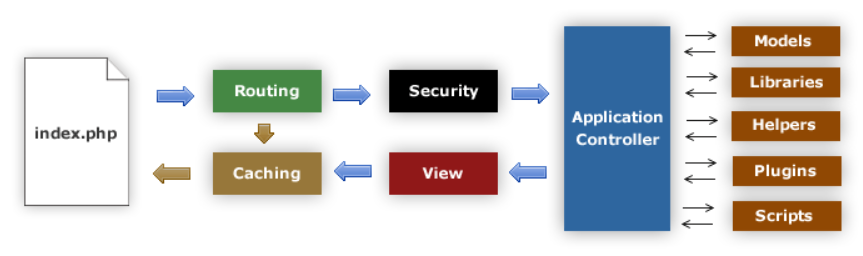
\includegraphics[scale=0.3]{ci3flowchart}  
	\caption[\textit{Flow Chart} Aplikasi \textit{CodeIgniter 3}]{\textit{Flow Chart} Aplikasi \textit{CodeIgniter 3}} 
	\label{fig:ci3flowchart} 
\end{figure} 

Berikut merupakan pembagian \textit{flow chart} aplikasi \textit{CodeIgniter 3}:
\begin{enumerate}
\item \texttt{index.php} berfungsi sebagai \textit{front controller} yang berguna untuk melakukan inisiasi
\item \textit{Router} berfungsi dalam melakukan pemeriksaan dan menentukan penggunaan \textit{HTTP Request}.
\item \textit{Cache} berfungsi untuk mengirimkan \textit{file cache}(apabila ada) kepada \textit{browser} secara langsung.   
\item \textit{Security} berfungsi sebagai alat penyaringan setiap data dan \textit{HTTP Request} yang masuk. Penyaringan data tersebut dilakukan sebelum \textit{controller} aplikasi dimuat agar aplikasi menjadi lebih aman.
\item \textit{Controller} berguna sebagai alat untuk memuat \textit{model, libraries}, dan sumber daya yang dibutuhkan untuk menjalankan permintaan spesifik.
\item \textit{View} akan dikirimkan menuju \textit{browser} untuk dilihat oleh pengguna. Apabila \textit{caching} dinyalakan, maka \textit{view} akan dilakukan \textit{cached} terlebih dahulu sehingga permintaan selanjutnya dapat diberikan.
\end{enumerate}

\subsection{\textit{Model-View-Controller}}
\textit{CodeIgniter 3} merupakan \textit{framework} berbasis arsitektur \textit{Model-View-Controller} atau yang selanjutnya akan disebut sebagai MVC. MVC merupakan sebuah pendekatan perangkat lunak yang memisahkan antara logika dengan presentasi atau tampilannya. Penggunaan struktur ini mengurangi penggunaan skrip pada halaman web karena tampilan terpisah dengan skrip PHP. Berikut merupakan penjelasan mengenai struktur MVC:

\subsubsection{\textit{\textbf{Model}}} \textit{Model} berfungsi dalam mewakili struktur data perangkat lunak. \textit{Model} berfungsi dalam mengambil, memasukan, dan memperbarui data pada \textit{database}. Berikut merupakan contoh \textit{file Model} \textit{CodeIgniter 3} pada direktori \verb|application/models/|:

\begin{lstlisting}[caption=Contoh \textit{model} pada \textit{CodeIgniter 3}, label=kode:model]
class Blog_model extends CI_Model {

        public $title;
        public $content;
        public $date;

        public function get_last_ten_entries()
        {
                $query = $this->db->get('entries', 10);
                return $query->result();
        }

        public function insert_entry()
        {
                $this->title    = $_POST['title']; // please read the below note
                $this->content  = $_POST['content'];
                $this->date     = time();

                $this->db->insert('entries', $this);
        }

        public function update_entry()
        {
                $this->title    = $_POST['title'];
                $this->content  = $_POST['content'];
                $this->date     = time();

                $this->db->update('entries', $this, array('id' => $_POST['id']));
        }

}
\end{lstlisting}

Kode \ref{kode:model} membentuk beberapa fungsi yaitu:
\begin{itemize}
\item \verb|get_last_ten_entries()| yang berfungsi untuk mengambil 10 data terakhir dari tabel \verb|entries| menggunakan \textit{query builder}.
\item \verb|insert_entry()| yang berfungsi untuk memasukan data \textit{title,content},dan \textit{date} menuju tabel \verb|entries|.
\item \verb|update_entry()| yang befungsi untuk memperbaharui data \textit{title,content},dan \textit{date} pada tabel \verb|entries| .
\end{itemize}
\textit{Model} biasanya digunakan pada \textit{file controller} dan dapat dipanggil menggunakan: 
\begin{center}
\verb|$this->load->model('model_name');|.
\end{center}

\subsubsection{\textit{\textbf{View}}} berfungsi dalam menyajikan informasi kepada pengguna. \textit{View} biasanya merupakan halaman web namun, pada \textit{CodeIgniter 3} \textit{view} dapat berupa pecahan halaman seperti \textit{header} atau \textit{footer}. Pecahan halaman dapat dimasukan pada halaman lain agar mempermudah dan membentuk kode yang lebih bersih.

\begin{lstlisting}[caption=Contoh \textit{view} pada \textit{CodeIgniter 3}, label=kode:view]
<?php
<html>
<head>
        <title>My Blog</title>
</head>
<body>
        <h1>Welcome to my Blog!</h1>
</body>
</html>
\end{lstlisting}

Kode \ref{kode:view} merupakan contoh \textit{file view} \textit{CodeIgniter 3} pada direktori \verb|application/views/| yang berisikan judul My Blog dan \textit{heading} Welcome to my Blog!. Pengguna dapat memanggil halaman yang sudah dibentuk pada \textit{file controller} dengan cara sebagai berikut:

\begin{center}
\verb|$this->load->view('name');|
\end{center}

\subsubsection{\textit{\textbf{Controller}}} berfungsi sebagai perantara antara \textit{Model}, \textit{View}, dan sumber daya yang dibutuhkan untuk melakukan proses \textit{HTTP Request} dan menjalankan halaman web. Penamaan \textit{controller} biasanya digunakan sebagai \textit{url} pada perangkat lunak pengguna. Berikut merupakan contoh \textit{controller} \textit{CodeIgniter 3} pada direktori \verb|application/controllers/|:

\begin{lstlisting}[caption=Contoh \textit{controller} pada \textit{CodeIgniter 3}, label=kode:controller]
<?php
class Blog extends CI_Controller {

        public function index()
        {
                echo 'Hello World!';
        }

        public function comments()
        {
                echo 'Look at this!';
        }
}
\end{lstlisting}

Kode \ref{kode:controller} berfungsi dalam mengembalikan \textit{string} sesuai dengan \textit{controller} yang dipanggil .Nama \textit{controller} dan metode diatas akan dijadikan segmen pada \textit{URL} seperti berikut:

\begin{center}
\verb|example.com/index.php/blog/index/|
\end{center}

Metode \textit{index} akan secara otomatis dipanggil menjadi \textit{URL} dan pengguna juga dapat memberi parameter untuk metode \textit{controller} yang nantinya akan menjadi \textit{URL}.

\iffalse
Overview bisa disatuin aja jadi epndahuluan (Flowchart and MVC).
General topic subsubbab.
Sisanya desesuain sama yg dipake Judge dan kalo ada bab yg bisa disatuin disatuin aja(libraries di general topic/helpers).
\textit{CodeIgniter 3} memiliki beragam fungsi untuk mempermudah pengguna dalam membentuk aplikasi web. Berikut merupakan fungsi-fungsi yang ada pada \textit{CodeIgniter 3}:
\fi

\subsection{\textit{CodeIgniter URLs}}

\textit{CodeIgniter 3} menggunakan pendekatan \textit{segment-based} dibandingkan menggunakan \textit{query string} untuk membentuk \textit{URL} yang mempermudah mesin pencari dan pengguna. Berikut merupakan contoh \textit{URL} pada \textit{CodeIgniter 3}:

\begin{center}
\verb|example.com/news/article/my_article|
\end{center}

Struktur segmen pada MVC menghasilkan \textit{URL} sebagai berikut :

\begin{center}
\verb|example.com/class/function/ID|
\end{center}

Segmen tersebut dibagi menjadi tiga buah yakni:
\begin{enumerate}
\item Segmen pertama mereprentasikan kelas \textit{controller} yang dipanggil.
\item Segmen kedua mereprentasikan kelas fungsi atau metode yang digunakan.
\item Segmen ketiga dan segmen lainnya mereprentasikan \textit{ID} dari variabel yang akan dipindahkan menuju \textit{controller}.
\end{enumerate}

Secara asali \textit{URL} yang dihasilkan \textit{CodeIgniter 3} terdapat nama \textit{file} \verb|index.php| seperti contoh dibawah ini:

\begin{center}
\verb|example.com/index.php/news/article/my_article|
\end{center}

Pengguna dapat menghapus \textit{file} \verb|index.php| file pada \textit{url} menggunakan \textit{file} \verb|.htaccess| apabila \textit{server Apache} pengguna menghidupkan \verb|mod_rewrite|. Berikut merupakan contoh \textit{file} \verb|.htaccess| menggunakan metode \textit{negative}:

\begin{lstlisting}[language=Java, caption=Contoh \textit{file} \texttt{.htaccess} pada halaman index.php, label=kode:htaccess]
RewriteEngine On
RewriteCond %{REQUEST_FILENAME} !-f
RewriteCond %{REQUEST_FILENAME} !-d
RewriteRule ^(.*)$ index.php/$1 [L]
\end{lstlisting}

Aturan diatas menyebabkan \textit{HTTP Request} selain yang berasal dari direktori atau \textit{file} diperlakukan sebagai sebuah permintaan pada file \verb|index.php|. Selain itu, pengguna juga dapat menambahkan akhirkan pada \textit{URL} agar halaman pengguna dapat menampilkan halaman sesuai dengan tipe yang diingikan. Berikut merupakan contoh \textit{URL} sebelum dan sesudah ditambahkan akhiran berupa: 

\begin{center}
\verb|example.com/index.php/products/view/shoes|

\verb|example.com/index.php/products/view/shoes.html|
\end{center}

Pengguna juga dapat menyalakan fitur \textit{query strings} dengan cara sebagai mengubah \textit{file application/config.php} seperti:

\begin{lstlisting}[caption=\textit{File application/config.php}, label=kode:querystring]
$config['enable_query_strings'] = FALSE;
$config['controller_trigger'] = 'c';
$config['function_trigger'] = 'm';
\end{lstlisting}

Pengguna dapat mengubah \verb|enable_query_strings| menjadi \textit{TRUE}. \textit{Controller} dan \textit{function} dapat diakses menggunakan kata yang sudah diatur.

\subsection{\textit{Helpers}}
\textit{Helpers} merupakan fungsi pada \textit{CodeIgniter 3}
yang mempermudah pengguna dalam membentuk aplikasi web. Setipa \textit{file helpers} terdiri dari banyak fungsi yang membantu sesuai kategori dan tidak ditulis dalanm format \textit{Object Oriented}. \textit{File helpers} terdapat pada direktori \textit{system/helpers} atau \textit{application/helpers}. Pengguna dapat memakai fitur \textit{helpers} dengan cara memuatnya seperti berikut:

\begin{center}
\verb|$this->load->helper('name');|
\end{center}

Pemanggilan \textit{helper} tidak menggunakan ekteksi .php melainkan hanya menggunakan nama dari \textit{helper} tersebut. Pengguna dapat memanggil satu atau banyak \textit{helper} pada metode \textit{controller} ataupun \textit{view} sesudah dimuat.

\subsection{\textit{Libraries}}
\textit{CodeIgniter 3} menyediakan \textit{library} yang dapat dipakai pengguna untuk mempermudah pembentukan aplikasi web. \textit{Library} merupakan kelas yang tersedia pada direktori \textit{application/libraries} dan dapat ditambahkan, diperluas, dan digantikan. 

\begin{lstlisting}[caption=Contoh kelas \textit{library} pada \textit{CodeIgniter 3}, label=kode:libraryclass]
<?php
defined('BASEPATH') OR exit('No direct script access allowed');

class Someclass {

        public function some_method()
        {
        }
}
\end{lstlisting}

Kode \ref{kode:libraryclass} merupakan contoh \textit{file library} pada \textit{CodeIgniter 3}. Setiap pembentukan \textit{file library} diperlukan huruf kapital dan harus sama dengan nama kelasnya. Berikut merupakan contoh pemanggilan \textit{file library} pada \textit{file controller}:

\begin{center}
\verb|$params = array('type' => 'large', 'color' => 'red');|

\verb|$this->load->library('someclass', $params);|
\end{center} 

Pemanggilan kelas ini dapat dilakukan melalui \textit{controller} manapun dan dapat diberikan parameter sesuai dengan metode yang dibentuk pada \textit{library}. \textit{CodeIgniter 3} menyediakan berbagai \textit{library} yang dapat digunakan oleh pengguna seperti berikut:

\subsubsection{\textit{JavaScript}}
Penggunaan kelas \textit{javascript} dapat dipanggil pada konstruktor \textit{controller} dengan cara berikut:

\begin{center}
\verb|$this->load->library('javascript');|
\end{center}

Pengguna selanjutnya harus melakukan inisiasi \textit{library} pada halaman \textit{view tag} \verb|<head>| seperti berikut:

\begin{center}
\verb|<?php echo $library_src;?>|

\verb|<?php echo $script_head;?>|
\end{center}

Sintaks \verb|$library_src| merupakan lokasi \textit{library} yang akan dimuat sedangkan \verb|$script_head| merupakan lokasi untuk fungsi yang akan dijalankan. Selanjutnya \textit{javascript} dapat diinisiasikan pada \textit{controller} menggunakan sintaks berikut:

\begin{center}
	\verb|$this->javascript|
\end{center}

Selain menggunakan \textit{javascript}, pengguna dapat memakai \textit{jQuery} dengan menambahkan \textit{jQuery} pada akhir inisiasi kelas \textit{javascript} seperti berikut:

\begin{center}
\verb|$this->load->library('javascript/jquery');|
\end{center}

Penggunga dapat memakai berbagai fungsi \textit{library jquery} menggunakan sintaks berikut:

\begin{center}
\verb|$this->jquery|
\end{center}

\subsubsection{Kelas \textit{Email}}
\textit{CodeIgniter 3} menyediakan kelas \textit{email} dengan fitur sebagai berikut:

\begin{itemize}
\item Beberapa Protokol: \textit{Mail, Sendmail}, dan \textit{SMTP}
\item Enkripsi \textit{TLS} dan \textit{SSL} untuk \textit{SMTP}
\item Beberapa Penerima
\item \textit{CC} dan \textit{BCCs}
\item \textit{HTML} atau \textit{email} teks biasa
\item Lampiran
\item Pembungkus kata
\item Prioritas
\item Mode\textit{BCC Batch}, memisahkan daftar \textit{email} besar menjadi beberapa \textit{BCC} kecil.
\item Alat \textit{Debugging email}
\end{itemize}

Penggunaan \textit{library email} dapat dikonfigurasikan pada \textit{file config}. Pengguna dapat mengirim \textit{email} dengan mudah menggunakan fungsi-fungsi yang telah disediakan \textit{library email}. Kode \ref{kode:emaillib} merupakan contoh pengiriman email melalui \textit{controller}.

\begin{lstlisting}[caption=Contoh pengiriman email melalui \textit{controller}, label=kode:emaillib]
$this->load->library('email');

$this->email->from('your@example.com', 'Your Name');
$this->email->to('someone@example.com');
$this->email->cc('another@another-example.com');
$this->email->bcc('them@their-example.com');

$this->email->subject('Email Test');
$this->email->message('Testing the email class.');

$this->email->send();
\end{lstlisting}

Kode \ref{kode:emaillib} merupakan contoh penggunaan \textit{library email} untuk mengirim \textit{email} dari \texttt{your@example.com} menuju \texttt{someone@example.com}. Konfigurasi ini juga mengirim dua buah salinan menuju \texttt{another@\\another-example.com} dan \texttt{them@their-example.com} dengan subjek berupa \texttt{Email Test} dengan pesan \texttt{Testing the email class.}. Selain itu, pengguna juga dapat melakukan konfigurasi preferensi \textit{email} melalui dua puluh satu preferesi. Pengguna dapat melakukan konfigurasi secara otomatis melalui \textit{file config} atau melakukan konfigurasi secara manual . Kode \ref{kode:emaillibset} merupakan contoh konfigurasi preferensi secara manual.

\begin{lstlisting}[caption=Contoh konfigurasi preferensi \textit{library email} secara manual, label=kode:emaillibset]
$config['protocol'] = 'sendmail';
$config['mailpath'] = '/usr/sbin/sendmail';
$config['charset'] = 'iso-8859-1';
$config['wordwrap'] = TRUE;

$this->email->initialize($config);
\end{lstlisting}
Kode \ref{kode:emaillibset} merupakan contoh konfigurasi pengiriman \textit{email} dengan protokol \texttt{sendmail} dan tujuan \texttt{usr/sbin/sendmail}.

\subsubsection{Kelas \textit{File Uploading}}
Pengunggahan \textit{file} terdapat empat buah proses sebagai berikut:
\begin{enumerate}
\item Dibentuk sebuah form untuk pengguna memilih dan mengunggah \textit{file}.
\item Setelah \textit{file} diunggah, \textit{file} akan dipindahkan menuju direktori yang dipilih.
\item Pada pengiriman dan pemindahan \textit{file} dilakukan validasi sesuai dengan ketentuan yang ada.
\item Setelah \textit{file} diterima akan dikeluarkan pesan berhasil.
\end{enumerate}

Perangkat lunak akan memindahkan \textit{file} yang sudah diunggah pada \textit{form} menuju \textit{controller} untuk dilakukan validasi dan penyimpanan.

\begin{lstlisting}[caption=Contoh \textit{controller} untuk melakukan validasi dan penyimpanan, label=kode:controllerfileupload]
<?php

class Upload extends CI_Controller {

        public function __construct()
        {
                parent::__construct();
                $this->load->helper(array('form', 'url'));
        }

        public function index()
        {
                $this->load->view('upload_form', array('error' => ' ' ));
        }

        public function do_upload()
        {
                $config['upload_path']          = './uploads/';
                $config['allowed_types']        = 'gif|jpg|png';
                $config['max_size']             = 100;
                $config['max_width']            = 1024;
                $config['max_height']           = 768;

                $this->load->library('upload', $config);

                if ( ! $this->upload->do_upload('userfile'))
                {
                        $error = array('error' => $this->upload->display_errors());

                        $this->load->view('upload_form', $error);
                }
                else
                {
                        $data = array('upload_data' => $this->upload->data());

                        $this->load->view('upload_success', $data);
                }
        }
}
?>
\end{lstlisting}

Kode \ref{kode:controllerfileupload} merupakan contoh kode dengan dua buah metode yakni:
\begin{enumerate}
\item \verb|index()| yang digunakan untuk mengembalikan \textit{view} bernama \texttt{upload\_form}
\item \verb|do_upload| yang digunakan untuk melakukan validasi berupa tipe, ukuran, lebar, dan panjang maksimal sebuah file. Metode ini juga mengembalikan \textit{error} dan menyimpan \textit{file} sesuai dengan direktori yang sudah diatur.
\end{enumerate}
Direktori penyimpanan dapat diubah sesuai dengan kebutuhan namun perlu pengubahan izin direktori menjadi 777 agar dapat di baca, di tulis, dan di eksekusi oleh seluruh pengguna.

\subsubsection{Kelas \textit{Zip Encoding}}
\textit{Zip} merupakan format sebuah \textit{file} yang berguna untuk melakukan kompress terhadap \textit{file} untuk mengurangi ukuran dan menjadikannya sebuah \textit{file}. \textit{CodeIgniter 3} menyediakan \textit{library Zip Encoding} yang dapat digunakan untuk membentuk arsip \textit{Zip} yang dapat diunduh menuju \textit{desktop} atau disimpan pada direktori. \textit{Library} ini dapat diinsiasi dengan kode sebagai berikut:

\begin{center}
\verb|$this->load->library('zip');|
\end{center}

Setelah diinisiasi, pengguna dapat memanggil \textit{library} tersebut menggunakan kode sebagai berikut:

\begin{center}
\verb|$this->zip|
\end{center}

Kode \ref{kode:zip} merupakan contoh penggunaan \textit{library Zip Encoding} untuk meyimpan dan menunduh data.

\begin{lstlisting}[caption=Contoh penggunaan \textit{library Zip Encoding}, label=kode:zip]
$name = 'mydata1.txt';
$data = 'A Data String!';

$this->zip->add_data($name, $data);

// Write the zip file to a folder on your server. Name it "my_backup.zip"
$this->zip->archive('/path/to/directory/my_backup.zip');

// Download the file to your desktop. Name it "my_backup.zip"
$this->zip->download('my_backup.zip');
\end{lstlisting}

Kode \ref{kode:zip} merupakan contoh untuk melakukan penyimpanan \textit{Zip file} pada direktori dan dapat mengunduh \textit{file} menuju \textit{desktop} pengguna. Selain menggunakan \textit{library} yang sudah disediakan, pengguna dapat membentuk dan memperluas \textit{libraries} sendiri sesuai dengan kebutuhan. Kode merupakan contoh \textit{library} yang dibentuk.

\begin{lstlisting}[caption=Contoh \textit{library} yang dibentuk, label=kode:newlib]
class Example_library {

        protected $CI;

        // We'll use a constructor, as you can't directly call a function
        // from a property definition.
        public function __construct()
        {
                // Assign the CodeIgniter super-object
                $this->CI =& get_instance();
        }

        public function foo()
        {
                $this->CI->load->helper('url');
                redirect();
        }
}
\end{lstlisting}

\textit{Library} diatas merupakan contoh \textit{library} yang dibentuk oleh pengguna digunakan untuk memanggil \textit{helper} bernama \textit{url}. Pengguna dapat memanggil kelas tersebut seperti memanggil kelas \textit{library} lainnya. Selain itu, pengguna juga dapat mengganti \textit{library} yang sudah ada dengan \textit{library} yang dibentuk pengguna dengan mengubah nama kelas sama persis dengan nama \textit{library} yang ingin digantikan.

\subsection{\textit{Database}}
\textit{CodeIgniter 3} memiliki konfigurasi \textit{database} yang menyimpan data-data terkait aturan \textit{database}.

\begin{lstlisting}[caption=Contoh konfigurasi \textit{database}, label=kode:databaseconf]
$db['default'] = array(
        'dsn'   => '',
        'hostname' => 'localhost',
        'username' => 'root',
        'password' => '',
        'database' => 'database_name',
        'dbdriver' => 'mysqli',
        'dbprefix' => '',
        'pconnect' => TRUE,
        'db_debug' => TRUE,
        'cache_on' => FALSE,
        'cachedir' => '',
        'char_set' => 'utf8',
        'dbcollat' => 'utf8_general_ci',
        'swap_pre' => '',
        'encrypt' => FALSE,
        'compress' => FALSE,
        'stricton' => FALSE,
        'failover' => array()
);
\end{lstlisting}

Kode \ref{kode:databaseconf} merupakan contoh konfigurasi pada file \textit{database} untuk \textit{database} bernama \texttt{database\_name} dengan \textit{username} \texttt{root} tanpa sebuah \textit{password}. \textit{CodeIgniter 3} menyediakan fitur \textit{query} untuk menyimpan, memasukan, memperbarui, dan menghapus data pada \textit{database} sesuai dengan konfigurasi \textit{database} yang sudah diatur. Kode \ref{kode:databaseselect} merupakan contoh \textit{query} untuk melakukan \textit{select} dan \textit{join} pada \textit{CodeIgniter 3}:

\begin{lstlisting}[caption=Contoh penggunaan \textit{query}, label=kode:databaseselect]
$this->db->select('*');
$this->db->from('blogs');
$this->db->join('comments', 'comments.id = blogs.id');
$query = $this->db->get();
\end{lstlisting}

Kode \ref{kode:databaseselect} merupakan contoh kode untuk melakukan \textit{query} pada tabel \texttt{blogs} yang melakukan \textit{join} dengan tabel \texttt{comments}. Pengguna dapat mengambil hasil dari \textit{query} menjadi \textit{object} atau \textit{array}. Selain itu, \textit{database} pada \textit{CodeIgniter 3} juga dapat digunakan untuk membentuk, menghapus, dan mengubah \textit{database} ataupun menambahkan kolom pada \textit{table}. Penggunaan \textit{database} untuk mebentuk, menghapus, atau mengubah \textit{database} harus dilakukan inisasi sebagai berikut:
\begin{center}
\verb|$this->load->dbforge()|
\end{center}
Setelah dilakukan inisiasi pengguna dapat membentuk \textit{database} menggunakan kelas \textit{Forge}. Kode \ref{kode:databasecreate} merupakan contoh untuk membentuk \textit{database}.

\begin{lstlisting}[caption=Contoh membentuk \textit{database} menggunakan \textit{CodeIgniter3} , label=kode:databasecreate]
	$this->dbforge->create_database('db_name')
\end{lstlisting}

Selain itu, pengguna juga dapat menambahkan kolom dengan konfigurasinya. Kode \ref{kode:databasefield} merupakan contoh penambahan kolom sesuai dengan kebutuhan pengguna.

\begin{lstlisting}[caption=Contoh menambahkan kolom dengan konfigurasinya menggunakan \textit{CodeIgniter3} , label=kode:databasefield]
	$fields = array(
        'blog_id' => array(
                'type' => 'INT',
                'constraint' => 5,
                'unsigned' => TRUE,
                'auto_increment' => TRUE
        ),
        'blog_title' => array(
                'type' => 'VARCHAR',
                'constraint' => '100',
                'unique' => TRUE,
        ),
        'blog_author' => array(
                'type' =>'VARCHAR',
                'constraint' => '100',
                'default' => 'King of Town',
        ),
        'blog_description' => array(
                'type' => 'TEXT',
                'null' => TRUE,
        ),
);
$this->dbforge->add_field($fields)
$this->dbforge->create_table('table_name');
\end{lstlisting}
Kode \ref{kode:databasefield} merupakan contoh penggunaan \textit{database} untuk menambahkan kolom sesuai dengan tipenya pada tabel \texttt{table\_name}.

\subsection{\textit{URI Routing}}
\textit{URL string} biasanya menggunakan nama atau metode \textit{controller} seperti pada berikut:

\begin{center}
\verb|example.com/class/function/id/|
\end{center}

Namun, pengguna dapat melakukan pemetaan ulang terhadap \textit{url} yang dibentuk agar dapat memanggil beberapa metode.

\begin{lstlisting}[caption=Contoh \textit{url} yang sudah dimetakan,label=kode:urlrouting]
example.com/product/1/
example.com/product/2/
example.com/product/3/
example.com/product/4/
\end{lstlisting}

Kode \ref{kode:urlrouting} merupakan contoh \textit{url} yang sudah dimetakan ulang. Pengguna dapat menambahkan kode pemetaan pada \textit{file application/config/routes.php} yang terdapat \textit{array} bernama \verb|$route|. Berikut merupakan beberapa cara melakukan pemetaan terhadap \textit{url}:

\subsubsection{WildCards}

\textit{Route wildcard} biasanya berisikan kode seperti berikut:

\begin{center}
\verb|$route['product/:num'] = 'catalog/product_lookup';|
\end{center}

\textit{Route} diatas dibagi menjadi dua buah yakni:
\begin{enumerate}
\item Bagian segmen \textit{URL}

Bagian pertama merupakan segmen pertama \textit{url} yang akan tampil pada \textit{url}. Bagian kedua merupakan segmen kedua dapat berisikan angka atau karakter.

\item Bagian kelas dan metode

Bagian kedua berisikan kelas dan metode dari \textit{controller} yang akan digunakan pada \textit{url}.

\end{enumerate} 

\subsubsection{Ekspresi Reguler}

Pengguna dapat memakai ekspresi reguler untuk melakukan pemetaan ulang \textit{route}. Berikut merupakan contoh ekspresi reguler yang biasa digunakan:

\begin{center}
\verb|$route['products/([a-z]+)/(\d+)'] = '$1/id_$2';|
\end{center}

Ekpresi ini menghasilkan \textit{URI} \textit{products/shirts/123} yang memanggil kelas \textit{controller} dan metode \textit{id\_123}. Pengguna juga dapat mengambil segmen banyak seperti berikut:
\begin{center}
\verb|$route['login/(.+)'] = 'auth/login/$1';|
\end{center}

\section{SharIF Judge\cite{sharif:23}}
\label{sec:judge}

\textit{SharIF Judge} merupakan sebuah \textit{Online Judge} percabangan dari \textit{Sharif Judge} yang dibentuk oleh Mohammed Javad Naderi. \textit{Sharif Judge} dibentuk menggunakan \textit{CodeIgniter 3} dan dimodifikasi sesuai dengan kebutuhan di Informatika Universitas Katolik Parahyangan menjadi nama \textit{SharIF Judge}. \textit{SharIF Judge} dapat menilai kode berbahasa \textit{C, C++, Java, dan Python} dengan mengunggah file ataupun mengetiknya langsung.

\subsection{Struktur Aplikasi}
\label{subsec:judgestructure}
\begin{lstlisting}
.
|-- application
|   |-- cache
|   |-- config
|   |-- controllers
|   |-- core
|   |-- core
|   |-- helpers
|   |-- hooks
|   |-- language
|   |-- libraries
|   |-- logs
|   |-- models
|   |-- third_party
|   |-- vendor
|   |-- views
|-- assets
|   |-- images
|   |-- js
|   |-- styles
|-- restricted
|   |-- tester
|-- system
\end{lstlisting}

\subsection{Instalasi}
\label{subsec:instalasi}

Berikut merupakan persyaratan dan langkah-langkah melakukan \textit{instalasi SharIF Judge}:

\subsubsection{Persyaratan}
\label{subsubsec:persyaratan}
SharIF Judge dapat dijalankan pada sistem operasi \textit{Linux} dengan syarat sebagai berikut:
\begin{itemize}
\item Diperlukan \textit{webserver} dengan versi PHP 5.3 atau lebih baru.
\item Pengguna dapat menjalankan PHP pada \textit{command line}. Pada \textit{Ubuntu} diperlukan instalasi paket \textit{php5-cli}.
\item \textit{MySql database} dengan ekstensi \textit{Mysqli} untuk PHP atau \textit{PostgreSql database}.
\item PHP harus memiliki akses untuk menjalankan perintah melalui fungsi \textit{shell\textunderscore exec}.

\begin{lstlisting}[language=Java, caption=Kode untuk melakukah pengetesan fungsi, label=kode:shell]
	echo shell_exec("php -v");
\end{lstlisting}

\item \textit{Tools} untuk melakukan kompilasi dan menjalankan kode yang dikumpulkan (\textit{gcc, g++, javac, java, python2, python3}).
\item \textit{Perl} disarankan untuk diinstalasi untuk alasan ketepatan waktu, batas memori, dan memaksimalkan batas ukuran pada hasil kode yang dikirim.
\end{itemize}

\subsubsection{Instalasi}
\begin{enumerate}
\item Mengunduh versi terakhir dari \textit{SharIF Judge} dan melakukan \textit{unpack} pada direktori \textit{public html}.
\item Memindahkan \textit{folder system} dan \textit{application} diluar direktori \textit{public} dan mengubah \textit{path} pada \verb|index.php|(Opsional).

\begin{lstlisting}[language=Java, caption=Contoh \textit{path} pada halaman index.php, label=kode:movesystemandapp]
	$system_path = '/home/mohammad/secret/system';
	application_folder = '/home/mohammad/secret/application';
	
\end{lstlisting}
\item Membentuk \textit{database MySql} atau \textit{PostgreSql} untuk \textit{SharIF Judge}. Jangan melakukan instalasi paket koneksi \textit{database} apapun untuk \textit{C, C++, Java,} atau \textit{Python}.
\item Mengatur koneksi \textit{database} pada \textit{file} \verb|application/config/database.example.php| dan menyimpannya dengan nama \verb|database.php|. Pengguna dapat menggunakan awalan untuk nama tabel.

\begin{lstlisting}[language=Java, caption=Contoh pengaturan koneksi untuk \textit{database}, label=kode:dbsetup]
/*  Enter database connection settings here:  */
'dbdriver' => 'postgre',    // database driver (mysqli, postgre)
'hostname' => 'localhost',  // database host
'username' => `,           // database username
'password' => `,           // database password
'database' => `,           // database name
'dbprefix' => 'shj_',       // table prefix
\end{lstlisting}
\item Mengatur \textit{RADIUS} \textit{server} dan \textit{mail server} pada \textit{file} \verb|application/config/secrets.example.php| dan menyimpannya dengan nama \verb|secrets.php|.
\item Mengatur \verb|application/cache/Twig| agar dapat ditulis oleh PHP.
\item Membuka halaman utama SharIF Judge pada \textit{web browser} dan mengikuti proses instalasi.
\item Melakukan \textit{Log in} dengan akun admin.
\item Memindahkan direktori \verb|tester| dan \verb|assignments| diluar direktori publik dan mengatur kedua direktori agar dapat ditulis oleh PHP. Selanjutnya Menyimpan \textit{path} kedua direktori pada halaman \textit{Settings}. Direktori \verb|assignments| digunakan untuk menyimpan \textit{file-file} yang diunggah agar tidak dapat diakses publik.

\end{enumerate}

\subsection{\textit{Clean URLs}}
\label{sec:cleanurls}
Secara asali, \verb|index.php| merupakan bagian dari seluruh \textit{urls} pada SharIF judge. Berikut merupakan contoh dari \textit{urls} SharIF Judge.

\begin{center}
\verb|http://example.mjnaderi.ir/index.php/dashboard|

\verb|http://example.mjnaderi.ir/index.php/users/add|
\end{center}

Pengguna dapat menghapus \verb|index.php| pada \textit{url} dan mendapatkan \textit{url} yang baik apabila sistem pengguna mendukung \textit{URL rewriting}.

\begin{center}
\verb|http://example.mjnaderi.ir/dashboard|

\verb|http://example.mjnaderi.ir/users/add|
\end{center}

\subsubsection{Cara Mengaktifkan \textit{Clean URLs}}
\begin{itemize}
\item Mengganti nama \textit{file} \verb|.htaccess2| pada direktori utama menjadi \verb|.htaccess|.
\item Mengganti \verb|$config['index_page'] = 'index.php';| menjadi \verb|$config['index_page'] = '';| pada \textit{file} \verb|application\config\config.php|.
\end{itemize}

\subsection{Users}
\label{sec:users}
Pada perangkat lunak SharIF Judge, pengguna dibagi menjadi 4 buah. Keempat pengguna tersebut adalah \textit{Admins, Head Instructors, Instructors}, dan\textit{ Students}. Tabel \ref{tab:userlevel} merupakan pembagian tingkat setiap pengguna.

\begin{table}[H]
	\centering 
	\caption{\textit{Tabel tingkat pengguna}}
	\label{tab:userlevel}
	\begin{tabular}{|c|c|}
		\hline
		\textit{\textbf{User Role}} & \textit{\textbf{User Level}} \\ \hline
		\textit{Admin} & 3 \\ \hline
		\textit{Head Instructor} & 2 \\ \hline
		\textit{Instructor} & 1 \\ \hline
		\textit{Student} & 0 \\ \hline		
	\end{tabular} 
\end{table}

Setiap pengguna memiliki akses untuk aksi yang berbeda berdasarkan tingkatnya. Tabel \ref{tab:userPermission} merupakan aksi yang dapat dilakukan oleh setiap pengguna.

\begin{table}[H] 
	\centering 
	\caption{\textit{Tabel izin aksi setiap pengguna}}
	\label{tab:userPermission}
	\begin{tabular}{|l|c|c|c|c|}
		\hline
		Aksi & \textit{Admin} & \textit{Head Instructor} & \textit{Instructor} & \textit{Student} \\
		
		\hline
		Mengubah \textit{Settings} & \ding{51} & \ding{53} & \ding{53} & \ding{53} \\
		Menambah/Menghapus Pengguna & \ding{51} & \ding{53} & \ding{53} & \ding{53} \\
		Mengubah Peran Pengguna & \ding{51} & \ding{53} & \ding{53} & \ding{53} \\
		Menambah/Menghapus/Mengubah \textit{Assignment} & \ding{51} & \ding{51} & \ding{53} & \ding{53} \\
		Mengunduh \textit{Test} & \ding{51} & \ding{51} & \ding{53} & \ding{53} \\
		
		Menambah/Menghapus/Mengubah Notifikasi & \ding{51} & \ding{51} & \ding{53} & \ding{53} \\
		\textit{Rejudge} & \ding{51} & \ding{51} & \ding{53} & \ding{53} \\
		Melihat/\textit{Pause}/Melanjutkan/\textit{Submission Queue} & \ding{51} & \ding{51} & \ding{53} & \ding{53} \\
		Mendeteksi Kode yang Mirip & \ding{51} & \ding{51} & \ding{53} & \ding{53} \\
		Melihat Semua Kode & \ding{51} & \ding{51} & \ding{51} & \ding{53} \\
		
		Mengunduh Kode Final& \ding{51} & \ding{51} & \ding{51} & \ding{53} \\
		Memilih \textit{Assignment} & \ding{51} & \ding{51} & \ding{51} & \ding{51} \\
		\textit{Submit} & \ding{51} & \ding{51} & \ding{51} & \ding{51} \\
		
		\hline
		
	\end{tabular} 
\end{table}

\subsubsection{Menambahkan Pengguna}

Admin dapat menambahkan pengguna melalui bagian \textit{Add User} pada halaman \textit{Users}. Admin harus mengisi setiap informasi dimana baris yang diawali \# merupakan komen dan setiap baris lainnya mewakili pengguna dengan sintaks berikut:
\begin{lstlisting}[language=Java, caption=Contoh sintaks untuk menambahkan pengguna, label=kode:addUser]
USERNAME,EMAIL,DISPLAY-NAME,PASSWORD,ROLE

* Usernames may contain lowercase letters or numbers and must be between 3 and 20 characters in length.
* Passwords must be between 6 and 30 characters in length.
* You can use RANDOM[n] for password to generate random n-digit password.
* ROLE must be one of these: `admin`, `head_instructor`, `instructor`, `student`
\end{lstlisting}

Dengan contoh sebagai berikut:
\begin{lstlisting}[language=Java, caption=Contoh kode untuk menambahkan pengguna, label=kode:addUserExample]
# This is a comment!
# This is another comment!
instructor,instructor@sharifjudge.ir,Instructor One,123456,head_instructor
instructor2,instructor2@sharifjudge.ir,Instructor Two,random[7],instructor
student1,st1@sharifjudge.ir,Student One,random[6],student
student2,st2@sharifjudge.ir,Student Two,random[6],student
student3,st3@sharifjudge.ir,Student Three,random[6],student
student4,st4@sharifjudge.ir,Student Four,random[6],student
student5,st5@sharifjudge.ir,Student Five,random[6],student
student6,st6@sharifjudge.ir,Student Six,random[6],student
student7,st7@sharifjudge.ir,Student Seven,random[6],student
\end{lstlisting}

\subsection{Menambah \textit{Assignment}}
\label{sec:addAssignment}
Pengguna dapat menambahkan \textit{assignment} baru melalui bagian \textit{Add} pada halaman \textit{Assignments}(dapat dilihat pada Gambar \ref{fig:addassignment}).
\begin{figure}[H]
	\centering  
	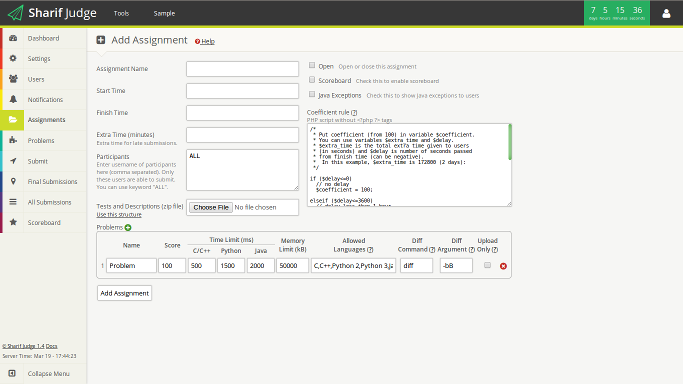
\includegraphics[scale=0.3]{addassignment}  
	\caption[Tampilan halaman \textit{SharIF Judge} untuk menambahkan \textit{assignment}]{Tampilan halaman \textit{SharIF Judge} untuk menambahkan \textit{assignment}} 
	\label{fig:addassignment} 
\end{figure} 

Berikut merupakan beberapa pengaturan pada halaman \textit{Add Assignments}:
\begin{itemize}
\item \subsubsection{\textit{Assignment Name}}
\textit{Assignment} akan ditampilkan sesuai dengan namanya pada daftar \textit{assignment}.

\item \subsubsection{\textit{Start Time}}
Pengguna tidak dapat mengumpulkan \textit{assignment} sebelum waktu dimulai("\textit{Start Time}"). Format pengaturan waktu untuk waktu mulai adalah \verb|MM/DD/YYYY HH:MM:SS| dengan contoh \verb|08/31/2013 12:00:00|. 

\item \subsubsection{\textit{Finish Time, Extra Time}}
Pengguna tidak dapat mengumpukan \textit{assignment} setelah \textit{Finish Time + Extra Time}. Pengumpulan \textit{Assignment} pada \textit{Extra Time} akan dikalikan seusai dengan koefisien. Pengguna harus menulis skrip PHP untuk menghitung koefisien pada \textit{field Coefficient Rule}. Format pengaturan waktu untuk waktu selesai sama seperti waktu mulai yakni \verb|MM/DD/YYYY HH:MM:SS| dan format waktu tambahan menggunakan menit dengan contoh \verb|120| (2 jam) atau \verb|48*60| (2 hari).  

\item \subsubsection{\textit{Participants}}
Pengguna dapat memasukan \textit{username} setiap partisipan atau menggunakan kata kunci \textit{ALL} untuk membiarkan seluruh pengguna melakukan pengumpulan. Contoh: \textit{admin, instructor1 , instructor2 ,student1  ,   student2,student3 , student4}.

\item \subsubsection{\textit{Tests}}
Pengguna dapat mengunggah \textit{test case} dalam bentuk \textit{zip file} sesuai dengan struktur pada \ref{subsec:testStructure}.

\item \subsubsection{\textit{Open}}
Pengguna dapat membuka dan menutup \textit{assigment} untuk pengguna \textit{student} melalui pilihan ini. Pengguna selain \textit{student} tetap dapat mengumpukan \textit{assignment} apabila sudah ditutup.

\item \subsubsection{\textit{Score Board}}
Pengguna dapat menghidupkan dan mematikan \textit{score board} melalui pilihan ini.

\item \subsubsection{\textit{Java Exceptions}}
Pengguna dapat menghidupkan dan mematikan fungsi untuk menunjukan \textit{java exceptions} kepada pengguna \textit{students} dan tidak akan memengaruhi kode yang sudah di \textit{judge} sebelumnya. Berikut merupakan tampilan apabila fitur \textit{java exceptions} dinyalakan:
\begin{lstlisting}[language=Java, caption=Contoh tampilan fitur \textit{Java Exceptions}, label=kode:javaexceptions]
Test 1
ACCEPT
Test 2
Runtime Error (java.lang.ArrayIndexOutOfBoundsException)
Test 3
Runtime Error (java.lang.ArrayIndexOutOfBoundsException)
Test 4
ACCEPT
Test 5
ACCEPT
Test 6
ACCEPT
Test 7
ACCEPT
Test 8
Runtime Error (java.lang.ArrayIndexOutOfBoundsException)
Test 9
Runtime Error (java.lang.StackOverflowError)
Test 10
Runtime Error (java.lang.ArrayIndexOutOfBoundsException)
\end{lstlisting}

\item \subsubsection{\textit{Archived Assignment}}
Pengguna dapat menghidupkan fitur ini dan \textit{assignment} akan dibentuk dengan waktu selesai \verb|2038-01-18 00:00:00| (UTC + 7) dengan kata lain pengguna memiliki waktut tidak terhingga untuk mengumpulkan \textit{assignment}.

\item \subsubsection{\textit{Coefficient Rule}}
Pengguna dapat menuliskan skrip PHP pada bagian ini untuk menghitung koefisien dikalikan dengan skor. Pengguna harus memasukan koefisien (dari 100) dalam variabel \verb|$coefficient|. Pengguna dapat menggunakan variabel \verb|$extra_time| dan \verb|$delay|. \verb|$extra_time| merupakan total dari waktu tambahan yang diberikan kepada pengguna dalam detik dan \verb|$delay| merupakan waktu dalam detik yang melewati waktu selesai(dapat berupa negatif). Skrip PHP pada bagian ini tidak boleh mengandung tag \verb|<?php|, \verb|<?|, dan \verb|?>|. Berikut merupakan contoh skrip dimana \verb|$extra_time| adalah 172800(2 hari):

\begin{lstlisting}[language=Java, caption=Contoh skrip PHP, label=kode:coefficientrule]
if ($delay<=0)
  // no delay
  $coefficient = 100;

elseif ($delay<=3600)
  // delay less than 1 hour
  $coefficient = ceil(100-((30*$delay)/3600));

elseif ($delay<=86400)
  // delay more than 1 hour and less than 1 day
  $coefficient = 70;

elseif (($delay-86400)<=3600)
  // delay less than 1 hour in second day
  $coefficient = ceil(70-((20*($delay-86400))/3600));

elseif (($delay-86400)<=86400)
  // delay more than 1 hour in second day
  $coefficient = 50;

elseif ($delay > $extra_time)
  // too late
  $coefficient = 0;
\end{lstlisting}

\item \subsubsection{\textit{Name}}
Merupakan nama dari masalah pada \textit{assignments}.

\item \subsubsection{\textit{Score}}
Merupakan skor dari masalah pada \textit{assignments}. 

\item \subsubsection{\textit{Time Limit}}
Pengguna dapat menentukan batas waktu untuk menjalankan kode dalam satuan milidetik. Bahasa \textit{Python} dan \textit{Java} biasanya memiliki waktu lebih lambat dari \textit{C/C++} sehingga membutuhkan waktu lebih lama.

\item \subsubsection{\textit{Memory Limit}}
Pengguna dapat menentukan batas memori dalam \textit{kilobytes} namun, pengguna pembatasan memori tidak terlalu akurat.

\item \subsubsection{\textit{Allowed Languages}}
Pengguna dapat menentukan bahasa setiap masalah pada \textit{assignment}(dipisahkan oleh koma). Terdapat beberapa bahasa yang tersedia yaitu \textit{C, C++, Java, Python 2, Python 3, Zip, PDF} ,dan \textit{TXT}. Pengguna dapat memakai \textit{Zip, PDF} ,dan \textit{TXT} apabila opsi \textit{Upload Only} dinyalakan. Contoh : \textit{C, C++, Zip} atau \textit{Python 2,Python 3}.

\item \subsubsection{\textit{Diff Command}}
\textit{Diff Command} digunakan untuk membandingkan keluaran dengan keluaran yang benar. Secara asali, \textit{SharIF Judge} menggunakan \verb|diff| namun, pengguna dapat menggantinya pada bagian ini dan bagian ini tidak boleh mengandung spasi.

\item \subsubsection{\textit{Diff Arguments}}
Pengguna dapat mengatur argumen untuk \textit{diff arguments} pada bagian ini. Pengguna dapat melihat \verb|man diff| untuk daftar lengkap argumen \textit{diff}. \textit{SharIF Judge} terdapat dua buah opsi baru yakni \verb|ignore| dan \verb|identical|.
\begin{itemize}
\item \verb|ignore| : \textit{SharIF Judge} mengabaikan semua baris baru dan spasi.
\item \verb|identical| : \textit{SharIF Judge} tidak mengabaikan apapun namun, keluaran dari \textit{file} yang dikumpulkan harus identik dengan \textit{test case} agar dapat diterima. 
\end{itemize}

\item \subsubsection{\textit{Upload Only}}
Pengguna dapat menghidupkan \textit{Upload only} namun, \textit{SharIF Judge} tidak akan menilai masalah tersebut. Pengguna dapat memakai \textit{ZIP}, \textit{PDF}, dan \textit{TXT} pada \textit{allowed languanges} apabila pengguna menghidupkan bagian ini.

\end{itemize}

\subsection{\textit{Sample Assignment}}
Berikut merupakan contoh dari \textit{assignment} untuk melakukan pengujian \textit{SharIF Judge}. Penambahan \textit{Assignment} dapat dilakukan dengan memencet tombol \textit{Add} pada halaman \textit{Assignment}.

\subsubsection{\textit{Problems}}
\begin{enumerate}
\item \textit{Problem 1 (Sum)}:
Program pengguna dapat membaca \textit{integer n}, membaca \textit{n integers} dan mengeluarkan hasil dari \textit{integer} tersebut.

\begin{table}[H]
\centering 
\label{tab:problem1}
\begin{tabular}{|l|c|}
\hline
\multicolumn{1}{|c|}{\textit{Sample Input}}             & \textit{Sample Output} \\ \hline
\begin{tabular}[c]{@{}l@{}}5\\ 53 78 0 4 9\end{tabular} & 145                    \\ \hline
\end{tabular}
\end{table}

\item \textit{Problem 2 (Max)}:
Program pengguna dapat membaca \textit{integer n}, membaca \textit{n integer}, dan mengeluarkan total dari dua buah \textit{integer} terbesar diantara \textit{n integer}.

\begin{table}[H]
\centering 
\label{tab:problem2}
\begin{tabular}{|l|c|}
\hline
\multicolumn{1}{|c|}{\textit{Sample Input}}                             & \textit{Sample Output} \\ \hline
\begin{tabular}[c]{@{}l@{}}7\\ 162 173 159 164 181 158 175\end{tabular} & 356                    \\ \hline
\end{tabular}
\end{table}

\item \textit{Problem 3 (Upload)}:
Pengguna dapat mengunggah \textit{file c} dan \textit{zip} dan \textit{problem} ini tidak akan dinilai karena hanya berupa \textit{Upload Only}.

\end{enumerate}

\subsubsection{Tests}
Pengguna dapat menemukan \textit{file zip} pada direktori \textit{Assignments}. Berikut merupakan susunan pohon dari ketiga \textit{problems} diatas:

\begin{lstlisting}
.
|-- p1
|   |-- in
|   |   |-- input1.txt
|   |   |-- input2.txt
|   |   |-- input3.txt
|   |   |-- input4.txt
|   |   |-- input5.txt
|   |   |-- input6.txt
|   |   |-- input7.txt
|   |   |-- input8.txt
|   |   |-- input9.txt
|   |   --- input10.txt
|   |-- out
|   |   --- output1.txt
|   |-- tester.cpp
|   --- desc.md
|-- p2
|   |-- in
|   |   |-- input1.txt
|   |   |-- input2.txt
|   |   |-- input3.txt
|   |   |-- input4.txt
|   |   |-- input5.txt
|   |   |-- input6.txt
|   |   |-- input7.txt
|   |   |-- input8.txt
|   |   |-- input9.txt
|   |   --- input10.txt
|   |-- out
|   |   |-- output1.txt
|   |   |-- output2.txt
|   |   |-- output3.txt
|   |   |-- output4.txt
|   |   |-- output5.txt
|   |   |-- output6.txt
|   |   |-- output7.txt
|   |   |-- output8.txt
|   |   |-- output9.txt
|   |   --- output10.txt
|   |-- desc.md
|   --- Problem2.pdf
|-- p3
|   --- desc.md
--- SampleAssignment.pdf
\end{lstlisting}

\textit{Problem 1} menggunakan metode \textit{"Tester"} untuk mengecek hasil keluaran, sehingga memiliki \textit{file} \verb|tester.cpp|(\textit{Tester Script}). \textit{Problem 2} mengguanakan metode \textit{"Output Comparison"} untuk mengecek hasil keluaran, sehingga memiliki dua buah direktori \textit{in} dan \textit{out} yang berisi \textit{test case}. \textit{Problem 3} merupakan \textit{problem "Upload-Only"}.

\subsubsection{\textit{Sample Solutions}}
Berikut merupakan \textit{sample solutions} untuk \textit{problem 1}:

Contoh solusi untuk bahasa \textit{C}
\begin{lstlisting}[language=C, caption=Contoh skrip PHP, label=kode:samplesolutions1]
#include<stdio.h>
int main(){
	int n;
	scanf("%d",&n);
	int i;
	int sum =0 ;
	int k;
	for(i=0 ; i<n ; i++){
		scanf("%d",&k);
		sum+=k;
	}
	printf("%d\n",sum);
	return 0;
}
\end{lstlisting}

Contoh solusi untuk bahasa \textit{C++}
\begin{lstlisting}[language=C, label=kode:samplesolutions2]
#include<stdio.h>
int main(){
	int n;
	scanf("%d",&n);
	int i;
	int sum =0 ;
	int k;
	for(i=0 ; i<n ; i++){
		scanf("%d",&k);
		sum+=k;
	}
	printf("%d\n",sum);
	return 0;
}
\end{lstlisting}

Contoh solusi untuk bahasa \textit{C}
\begin{lstlisting}[language=Java, label=kode:samplesolutions3]
import java.util.Scanner;
class sum
{
	public static void main(String[] args)
	{ 
		Scanner sc = new Scanner(System.in);
		int n = sc.nextInt();
		int sum =0;
		for (int i=0 ; i<n ; i++)
		{
			int a = sc.nextInt();
			sum += a;
		}
		System.out.println(sum); 
	}
}
\end{lstlisting}

Berikut merupakan contoh solusi untuk \textit{problem 2}:

Contoh solusi untuk bahasa \textit{C++}
\begin{lstlisting}[language=C,label=kode:samplesolutions21]
#include<stdio.h>
int main(){
	int n , m1=0, m2=0;
	scanf("%d",&n);
	for(;n--;){
		int k;
		scanf("%d",&k);
		if(k>=m1){
			m2=m1;
			m1=k;
		}
		else if(k>m2)
			m2=k;
	}
	printf("%d",m1+m2);
	return 0;
}
\end{lstlisting}

contoh solusi untuk bahasa \textit{C++}
\begin{lstlisting}[language=C,, label=kode:samplesolutions22]
#include<iostream>
using namespace std;
int main(){
	int n , m1=0, m2=0;
	cin >> n;
	for(;n--;){
		int k;
		cin >> k;
		if(k>=m1){
			m2=m1;
			m1=k;
		}
		else if(k>m2)
			m2=k;
	}
	cout << (m1+m2) << endl ;
	return 0;
}
\end{lstlisting}

\subsection{\textit{Test Structure}}
\label{subsec:testStructure}
Penambahan \textit{assignment} harus disertakan dengan \textit{file zip} berisikan \textit{test cases}. \textit{File zip} ini sebaiknya berisikan \textit{folder} untuk setiap masalah dengan nama \textit{p1,p1} dan \textit{p3} selain masalah \textit{Upload-Only}.

\subsubsection{Metode Pemeriksaan}
Terdapat dua buah metode untuk melakukan pemeriksaan yakni metode \textit{Input Output} dan metode \textit{Tester}.

\begin{enumerate}
\item Metode perbandingan \textit{Input Output}

Pada metode ini, pengguna harus memberi masukan dan keluaran pada \textit{folder problem}. Perangkat lunak akan memberikan \textit{file test input} ke kode pengguna dan melakukan perbandingan dengan hasil keluaran kode pengguna. \textit{File input} harus berada didalam \textit{folder in} dengan nama \textit{input1.txt, input2.txt}, dst. \textit{File output} harus berada di dalam \textit{folder out} dengan nama \textit{output1.txt,output2.txt}.

\item Metode perbandingan \textit{Tester}

Pada metode ini, pengguna harus menyediakan \textit{file input test,} sebuah \textit{file C++,} dan \textit{file output test}(opsional). Perangkat lunak akan memberikan \textit{file input test} ke kode pengguna dan mengambil keluaran pengguna. Selanjutnya, \verb|tester.cpp| akan mengambil masukan pengguna, keluaran tes dan keluaran program pengguna. Jika keluaran pengguna benar maka perangkat lunak akan mengembalikan 1 sedangkan apabila salah maka perangkat lunak akan mengembalikan 0. Berikut adalah templat yang dapat digunakan pengguna untuk menuliskan \textit{file} \textit{tester.cpp}:

\begin{lstlisting}[language=C,caption=Templat kode \textit{tester.cpp}, label=kode:cpptemplate]
/*
 * tester.cpp
 */
 
#include <iostream>
#include <fstream>
#include <string>
using namespace std;
int main(int argc, char const *argv[])
{
 
	ifstream test_in(argv[1]);    /* This stream reads from test's input file   */
	ifstream test_out(argv[2]);   /* This stream reads from test's output file  */
	ifstream user_out(argv[3]);   /* This stream reads from user's output file  */
 
	/* Your code here */
	/* If user's output is correct, return 0, otherwise return 1       */
 
	...
 
}
\end{lstlisting}

\subsubsection{\textit{Sample File}}
Pengguna dapat menemukan \textit{file sample test} pada direktori \textit{assignments}. Berikut merupakan contoh dari pohon \textit{file} tersebut:

\begin{lstlisting}
.
|-- p1
|   |-- in
|   |   |-- input1.txt
|   |   |-- input2.txt
|   |   |-- input3.txt
|   |   |-- input4.txt
|   |   |-- input5.txt
|   |   |-- input6.txt
|   |   |-- input7.txt
|   |   |-- input8.txt
|   |   |-- input9.txt
|   |   --- input10.txt
|   |-- out
|   |   --- output1.txt
|   |-- tester.cpp
|-- p2
|   |-- in
|   |   |-- input1.txt
|   |   |-- input2.txt
|   |   |-- input3.txt
|   |   |-- input4.txt
|   |   |-- input5.txt
|   |   |-- input6.txt
|   |   |-- input7.txt
|   |   |-- input8.txt
|   |   |-- input9.txt
|   |   --- input10.txt
|   |-- out
|   |   |-- output1.txt
|   |   |-- output2.txt
|   |   |-- output3.txt
|   |   |-- output4.txt
|   |   |-- output5.txt
|   |   |-- output6.txt
|   |   |-- output7.txt
|   |   |-- output8.txt
|   |   |-- output9.txt
|   |   --- output10.txt
\end{lstlisting}

\textit{Problem 1} menggunakan metode perbandingan \textit{Tester}, sehingga memiliki \textit{file tester.cpp}. Berikut merupakan \textit{file} untuk \textit{problem 1}:

\begin{lstlisting}[language=C,caption=Kode metode perbandingan \textit{tester} dengan bahasa \textit{tester.cpp}, label=kode:cppfileproblem1]
/*
 * tester.cpp
 */
 
#include <iostream>
#include <fstream>
#include <string>
using namespace std;
int main(int argc, char const *argv[])
{
 
	ifstream test_in(argv[1]);    /* This stream reads from test's input file   */
	ifstream test_out(argv[2]);   /* This stream reads from test's output file  */
	ifstream user_out(argv[3]);   /* This stream reads from user's output file  */
 
	/* Your code here */
	/* If user's output is correct, return 0, otherwise return 1       */
	/* e.g.: Here the problem is: read n numbers and print their sum:  */
 
	int sum, user_output;
	user_out >> user_output;
 
	if ( test_out.good() ) // if test's output file exists
	{
		test_out >> sum;
	}
	else
	{
		int n, a;
		sum=0;
		test_in >> n;
		for (int i=0 ; i<n ; i++){
			test_in >> a;
			sum += a;
		}
	}
 
	if (sum == user_output)
		return 0;
	else
		return 1;
 
}
\end{lstlisting}

\textit{Problem 2} menggunakan metode perbandingan \textit{Input Output} sehingga memiliki \textit{folder in} dan \textit{folder out} berisikan \textit{test case}. Sedangkan \textit{problem 3} merupakan \textit{Upload Only}, sehingga tidak memiliki \textit{folder} apapun.

\end{enumerate}

\subsection{Deteksi Kecurangan}
\textit{SharIF Judge} menggunakan \textit{Moss} untuk mendeteksi kode yang mirip. \textit{Moss}(\textit{Measure of Software Similarity}) merupakan sistem otomatis untuk menentukan kesamaan atau kemiripan dalam program. Penggunaan utama \textit{Moss} adalah untuk melakukan pemeriksaan plagiarisme pada kelas \textit{programming}. Pengguna dapat mengirim hasil kode terakhir(\textit{Final Submission}) ke \textit{server Moss} dengan satu klik.

Penggunaan \textit{Moss} memiliki beberapa hal yang harus diatur oleh pengguna yakni:

\begin{enumerate}
\item Pengguna harus mendapatkan \textit{Moss User id} dan melakukan pengaturan pada \textit{SharIF Judge}. Untuk mendapatkan \textit{Moss User id}, pengguna dapat mendaftar pada halaman \url{http://theory.stanford.edu/~aiken/moss/}. Pengguna selanjutkan akan mendapatkan \textit{email} berupa skrip \textit{perl} berisikan \textit{user id} pengguna. Berikut merupakan contoh dari potongan skrip \textit{perl}:

\begin{lstlisting}[language=C,caption=Contoh potongan skrip \textit{perl}, label=kode:perlexample]

...

$server = 'moss.stanford.edu';
$port = '7690';
$noreq = "Request not sent.";
$usage = "usage: moss [-x] [-l language] [-d] [-b basefile1] ... [-b basefilen] [-m #] [-c \"string\"] file1 file2 file3 ...";

#
# The userid is used to authenticate your queries to the server; don't change it!
#
$userid=YOUR_MOSS_USER_ID;

#
# Process the command line options.  This is done in a non-standard
# way to allow multiple -b's.
#
$opt_l = "c";   # default language is c
$opt_m = 10;
$opt_d = 0;

...

\end{lstlisting}
\textit{User id} pada skrip \textit{perl} diatas dapat digunakan pada \textit{SharIF Judge} untuk mendeteksi kecurangan. Pengguna dapat menyimpan \textit{user id} pada halaman \textit{SharIF Judge Moss} dan \textit{SharIF Judge} akan menggunakan \textit{user id} tersebut.

\item \textit{Server} pengguna harus memiliki instalasi \verb|perl| untuk menggunakan \textit{Moss}.
\item Pengguna dianjurkan untuk mendeteksi kode yang mirip setelah \textit{assignment} selesai karena \textit{SharIF Judge} akan mengirimkan hasil akhir kepada \textit{Moss} dan pengguna(\textit{students}) dapat mengganti hasil akhir sebelum \textit{assignment} selesai.

\end{enumerate}

\subsection{Keamanan}
Berikut merupakan langkah untuk melakukan pengaturan keamanan \textit{SharIF Judge}:
\begin{enumerate}
\item \subsubsection{Menggunakan \textit{Sandbox}}
Pengguna harus memastikan untuk menggunakan \textit{sandbox} untuk bahasa \textit{C/C++} dan menyalakan \textit{Java Security Manager (Java Policy)} untuk bahasa \textit{java}. Untuk menggunakan \textit{sandbox} dapat dilihat pada sub bab \ref{subsec:sandboxing}.

\item \subsubsection{Menggunakan \textit{Shield}}
Pengguna harus memastikan untuk menggunakan \textit{shield} untuk bahasa \textit{C, C++,} dan \textit{Python}. Penggunaan \textit{shield} dapat dilihat pada subbab \ref{subsec:shield}.

\item \subsubsection{Menjalankan sebagai \textit{Non-Priviledge User}}
Pengguna diwajibkan menjalankan kode yang telah dikumpulkan sebagai \textit{non-priviledge user}. \textit{Non-Priviledge User} adalah \textit{user} yang tidak memiliki akses jaringan, tidak dapat menulis \textit{file} apapun, dan tidak dapat membentuk banyak proses.

Diasumsikan bahwa PHP dijalankan sebagai pengguna \verb|www-data| pada server. Membentuk \textit{user} baru \verb|restricted-user| dan melakukan pengaturan \textit{password}. Selanjutnya, jalankan \verb|sudo visudo| dan tambahkan kode \verb|www-data ALL=(restricted_user) NOPASSWD: ALL| pada baris terakhir \textit{file sudoers}.
\begin{itemize}

\item Pada \textit{file} \verb|tester\runcode.sh| ubah kode:

\begin{lstlisting}[language=C,caption=Kode \textit{runcode.sh} awal, label=kode:runcodebefore]
if $TIMEOUT_EXISTS; then
	timeout -s9 $((TIMELIMITINT*2)) $CMD <$IN >out 2>err
else
	$CMD <$IN >out 2>err        
fi
\end{lstlisting}

menjadi:
\begin{lstlisting}[language=C,caption=Kode \textit{runcode.sh} awal, label=kode:runcodeafter]
if $TIMEOUT_EXISTS; then
	sudo -u restricted_user timeout -s9 $((TIMELIMITINT*2)) $CMD <$IN >out 2>err
else
	sudo -u restricted_user $CMD <$IN >out 2>err        
fi
\end{lstlisting}

dan \textit{uncomment} baris berikut:

\begin{lstlisting}[language=C,caption=Kode \textit{runcode.sh} awal, label=kode:runcodeuncomment]
sudo -u restricted_user pkill -9 -u restricted_user
\end{lstlisting}

\item Mematikan akses jaringan untuk \textit{restricted\char`_user}

Pengguna dapat mematikan akses jaringan untuk \textit{restricted\char`_user} di \textit{linux} menggunakan \textit{iptables}. Setelah dimatikan lakukan pengujian menggunakan \verb|ping| sebagai \textit{restricted\char`_user}.

\item Menolak izin menulis

Pastikan tidak ada direktori atau \textit{file} yang dapat ditulis oleh \textit{restricted\char`_user}.

\item Membatasi jumlah proses

Pengguna dapat membatasi jumlah proses dari \textit{restricted\char`_user} dengan menambahkan kode dibawah melalui \textit{file /etc/security/limits.conf}.

\begin{lstlisting}[caption=Contoh kode untuk membatasi jumlah proses, label=kode:limitprocess]
restricted_user     soft    nproc   3
restricted_user     hard    nproc   5
\end{lstlisting}

\end{itemize}

\item \subsubsection{Menggunakan dua \textit{server}}
Pengguna dapat memakai dua \textit{server} untuk antar muka web dan menangani permintaan web dan mengguna \textit{server} lainnya untuk menjalankan kode yang sudah dikumpulkan. Penggunaan dua \textit{server} mengurangi risiko menjalankan kode yang sudah dikumpulkan. Pengguna harus mengganti \textit{source code SharIF Judge} untuk memakai hal ini.

\end{enumerate}

\subsection{\textit{Sandboxing}}
\label{subsec:sandboxing}
\textit{SharIF Judge} menjalankan banyak \textit{arbitrary codes} yang pengguna kumpulkan. \textit{SharIF Judge} harus menjalankan kode pada lingkungan terbatas sehingga memerlukan perkakas untuk \textit{sandbox} kode yang sudah dikumpulkan. Pengguna dapat meningkatkan keamanan dengan menghidupkan \textit{shield} dan \textit{Sandbox}.

\subsubsection{\textit{C/C++ Sandboxing}}
\textit{SharIF Judge} menggunakan \textit{EasySandbox} untuk melakukan \textit{sandboxing} kode \textit{C/C++}. \textit{EasySandbox} berguna untuk membatasi kode yang berjalan menggunakan \textit{seccomp}. \textit{Seccomp} merupakan mekanisme \textit{sandbox} pada \textit{Linux kernel}. Secara asali \textit{EasySandbox} dimatikan pada \textit{SharIF Judge} namun, pengguna dapat menghidupkannya melalui halaman \textit{Settings}. Selain itu, pengguna juga harus \textit{"build EasySandbox"} sebelum menyalakannya. Berikut merupakan cara melakukan \textit{build EasySandbox}:

\textit{File EasySandbox} terdapat pada \textit{tester/easysandbox}. Untuk membangun \textit{EasySandbox} jalankan:

\begin{lstlisting}[language=C,caption=Kode \textit{runcode.sh} awal, label=kode:easysandbox]
$ cd tester/easysandbox
$ chmod +x runalltests.sh
$ chmod +x runtest.sh
$ make runtests
\end{lstlisting}

Jika keluaran berupa \textit{message All test passed!} maka, \textit{EasySandbox} berhasil dibangun dan dapat dinyalakan pada perangkat lunak.

\subsubsection{\textit{Java Sandboxing}}
Secara asali, \textit{Java Sandbox} sudah dinyalakan menggunakan \textit{Java Security Manager}. Pengguna dapat menghidupkan atau mematikannya pada halaman \textit{Settings}.

\subsection{\textit{Shield}}
\label{subsec:shield}
\textit{Shield} merupakan mekanisme sangat simpel untuk melarang jalannya kode yang berpotensi berbahaya. \textit{Shield} bukan solusi \textit{sanboxing} karena \textit{shield} hanya menyediakan proteksi sebagian terhadap serangan remeh. Proteksi utama terhadap kode tidak terpercaya adalah dengan menghidupkan \textit{Sandbox}(dapat dilihat pada subbab\ref{subsec:sandboxing}).

\subsubsection{\textit{Shield} untuk \textit{C/C++}}
Dengan menghidupkan \textit{shield} untuk \textit{c/c++}, \textit{SharIF Judge} hanya perlu menambahkan \verb|#define| pada awal kode yang dikumpulkan sebelum menjalankannya. Sebagai contoh, pengguna dapat melarang penggunaan \verb|goto| dengan menambahkan kode dibawah pada awal kode yang sudah dikumpulkan.
\begin{lstlisting}[language=C,caption=Kode \textit{shield} untuk melarang penggunaan goto, label=kode:goto]
#define goto YouCannotUseGoto
\end{lstlisting}
Dengan kode diatas, semua kode yang menggunakan \verb|goto| akan mendapatkan \textit{compilation error}. Apabila pengguna menghidupkan \textit{shield}, semua kode yang mengandung \verb|#undef| akan mendapatkan \textit{compilation error}.

\begin{itemize}
\item Menghidupkan \textit{shield} untuk \textit{C/C++}

Pengguna dapat menghidupkan atau mematikan \textit{shield} pada halaman \textit{settings}.

\item Menambahkan aturan untuk \textit{C/C++}
Daftar aturan \verb|#define| untuk bahasa \textit{C} terdapat pada halaman \textit{tester/shield/defc.h} dan \textit{tester/shield/defcpp.h} untuk bahasa \textit{C++}. Pengguna dapat menambahkan aturan baru pada \textit{file} tersebut pada halaman \textit{settings}. Berikut merupakan contoh sintaks pada untuk menambahkan aturan :

\begin{lstlisting}[language=C,caption=Sintaks aturan \textit{\#define}, label=kode:define]
/*

@file defc.h
There should be a newline at end of this file.
Put the message displayed to user after // in each line

e.g. If you want to disallow goto, add this line:
#define goto errorNo13    //Goto is not allowd

*/

#define system errorNo1      //"system" is not allowed
#define freopen errorNo2     //File operation is not allowed
#define fopen errorNo3       //File operation is not allowed
#define fprintf errorNo4     //File operation is not allowed
#define fscanf errorNo5      //File operation is not allowed
#define feof errorNo6        //File operation is not allowed
#define fclose errorNo7      //File operation is not allowed
#define ifstream errorNo8    //File operation is not allowed
#define ofstream errorNo9    //File operation is not allowed
#define fork errorNo10       //Fork is not allowed
#define clone errorNo11      //Clone is not allowed
#define sleep errorNo12      //Sleep is not allowed
\end{lstlisting}

Pada akhir baris \textit{file} \verb|defc.h| dan \verb|defcpp.h| harus terdapat baris baru. Terdapat banyak aturan yang tidak dapat digunakan pada \textit{g++}, seperti aturan \verb|#define fopen errorNo3| untuk bahasa \textit{C++}.

\end{itemize} 
\subsubsection{\textit{Shield} untuk \textit{Python}}

Penggunaan \textit{shield} untuk \textit{python} dapat dihidupkan melalui halaman \textit{settings}. Dengan menghidupkan \textit{shield} untuk \textit{python}, \textit{SharIF Judge} hanya menambahkan beberapa kode pada baris awal kode yang sudah dikumpulkan sebelum dijalankan. Penambahan kode digunakan untuk mencegah pemakaian fungsi berbahaya. Kode-kode tersebut terletak pada \textit{file tester/shield/shield\_py2.py} dan \textit{tester/shield/shield\_py3.py}. Berikut merupakan cara untuk keluar dari \textit{shield} untuk \textit{python} menggunakan fungsi yang telah di daftar hitamkan:

\begin{lstlisting}[language=Python,caption=Cara keluar dari \textit{shield} untuk \textit{python},label=kode:pythonshield]

# @file shield_py3.py

import sys
sys.modules['os']=None

BLACKLIST = [
  #'__import__', # deny importing modules
  'eval', # eval is evil
  'open',
  'file',
  'exec',
  'execfile',
  'compile',
  'reload',
  #'input'
  ]
for func in BLACKLIST:
  if func in __builtins__.__dict__:
    del __builtins__.__dict__[func]
    
\end{lstlisting}

\section{CodeIgniter 4\cite{codeigniter:23:ci4}}
\label{sec:ci4}

\textit{CodeIgniter 4} merupakan versi terbaru dari \textit{framework} \textit{CodeIgniter} yang berfungsi untuk membantu pembentukan web. \textit{CodeIgniter 4} dapat dipasang menggunakan \textit{composer} ataupun dipasang secara manual dengan mengunduhnya dari situs web resmi. Setelah dilakukan pemasangan \textit{CodeIgniter 4} memiliki lima buah direktori dengan struktur aplikasi sebagai berikut:

\begin{itemize}
\item \texttt{app/}

Direktori \textit{app} berisikan semua kode yang dibutuhkan untuk menjalankan aplikasi web yang dibentuk. Direktori ini memiliki beberapa direktori didalamnya yaitu:
\begin{itemize}
\item \verb|Config/| berfungsi dalam menyimpan \textit{file} konfigurasi aplikasi web pengguna.
\item \verb|Controllers/| berfungsi sebagai penentu alur program yang dibentuk.
\item \verb|Database/| berfungsi sebagai penyimpan \textit{file migrations} dan \textit{seeds}.
\item \verb|Filters/| befungsi dalam menyimpan \textit{file} kelas \textit{filter}.
\item \verb|Helpers/| berfungsi dalam menyimpan koleksi fungsi mandiri.
\item \verb|Language/| berfungsi sebagai tempat penyimpanan \textit{string} dalam berbagai bahasa.
\item \verb|Libraries/| berfungsi dalam penyimpan kelas yang tidak termasuk kategori lain.
\item \verb|Models/| berfungsi untuk merepresentasikan data dari \textit{database}.
\item \verb|ThirdParty/| \textit{library ThridParty} yang dapat digunakan pada aplikasi.
\item \verb|Views/| berisikan \textit{file HTML} yang akan ditampilkan kepada pengguna.
\end{itemize}

\item \texttt{public/}

Direktori \textit{public} merupakan \textit{web root} dari situs dan berisikan data-data yang dapat diakses oleh pengguna melalui \textit{browser}. Direktori ini berisikan \textit{file} \verb|.htaccess|, \verb|index.php|, dan \textit{assets} dari aplikasi web yang dibentuk seperti gambar, \textit{CSS}, ataupun \textit{JavaScript}.

\item \texttt{writable/}

Direktori \textit{writable} berisikan data-data yang mungkin perlu ditulis seperti \textit{file cache},\textit{logs}, dan \textit{uploads}. Pengguna dapat menambahkan direktori baru sesuai dengan kebutuhan sehingga menambahkan keamanan pada direktori utama.

\item \texttt{tests/}

Direktori ini menyimpan \textit{file} test dan tidak perlu dipindahkan ke \textit{server} produksi. Direktori \verb|_support| berisikan berbagai jenis kelas \textit{mock} dan keperluan yang dapat dipakai pengguna dalam menulis \textit{tests}.

\item \texttt{vendor/} atau \texttt{system/}

Direktori ini berisikan \textit{file} yang diperlukan dalam menjalani \textit{framework} dan tidak boleh dimodifikasi oleh pengguna. Pengguna dapat melakukan \textit{extend} atau membentuk kelas baru untuk menambahkan fungsi yang diperlukan.

\end{itemize}

\subsection{\textit{Models-Views-Controllers}}
\textit{CodeIgniter 4} menggunakan pola \textit{MVC} untuk mengatur \textit{file} agar lebih simpel dalam menemukan \textit{file} yang diperlukan. MVC menyimpan data, presentasi, dan alur program dalam \textit{file} yang berbeda.

\subsubsection{\textit{Models}}

\textit{Models} berfungsi dalam menyimpan dan mengambil data dari tabel spesifik pada \textit{database}. Data tersebut dapat berupa pengguna, pemberitahuan blog, transaksi, dll. \textit{Models} pada umumnya disimpan pada direktori \texttt{app/Models} dan memiliki \textit{namespace} sesuai dengan lokasi dari \textit{file} tersebut. Kode \ref{kode:modelsexample} merupakan contoh dari \textit{models}.

\begin{lstlisting}[caption=Contoh \textit{Models},label=kode:modelsexample]

<?php

namespace App\Models;

use CodeIgniter\Model;

class UserModel extends Model
{
    protected $table      = 'users';
    protected $primaryKey = 'id';

    protected $useAutoIncrement = true;

    protected $returnType     = 'array';
    protected $useSoftDeletes = true;

    protected $allowedFields = ['name', 'email'];

    // Dates
    protected $useTimestamps = false;
    protected $dateFormat    = 'datetime';
    protected $createdField  = 'created_at';
    protected $updatedField  = 'updated_at';
    protected $deletedField  = 'deleted_at';

    // Validation
    protected $validationRules      = [];
    protected $validationMessages   = [];
    protected $skipValidation       = false;
    protected $cleanValidationRules = true;

}
    
\end{lstlisting}

Kode \ref{kode:modelsexample} merupakan contoh \textit{Models} yang dapat digunakan pada \textit{controllers}. \textit{Models} tersebut terkoneksikan dengan tabel \texttt{users} dengan \textit{primarykey} \texttt{id}. \textit{Model} pada \textit{CodeIgniter 4} juga dapat digunakan untuk mencari, menyimpan, dan menghapus data untuk setiap tabel spesifik. Kode \ref{kode:modelfindall} merupakan contoh penggunaan \textit{model} untuk mencari data spesifik.
\begin{lstlisting}[caption=Contoh penggunaan \textit{model} untuk mencari data spesifik,label=kode:modelfindall]
<?php

$users = $userModel->where('active', 1)->findAll();
\end{lstlisting}

Kode \ref{kode:modelfindall} menggabungkan \textit{query} dengan metode pencarian \textit{model} untuk mencari seluruh data \verb|active|.

\subsubsection{\textit{Views}}

\textit{Views} merupakan halaman berisikan \textit{HTML} dan sedikit PHP yang ditampilkan kepada pengguna ataupun dapat berupa pecahan halaman seperti \textit{header, footer}, ataupun \textit{sidebar}. \textit{Views} biasanya terdapat pada \verb|app/Views| dan mendapatkan data berupa variabel dari \textit{controller} untuk ditampilkan.

\begin{lstlisting}[caption=Contoh \textit{Views},label=kode:viewsexample]
<html>
    <head>
        <title>My Blog</title>
    </head>
    <body>
        <h1>Welcome to my Blog!</h1>
    </body>
</html>
\end{lstlisting}

Kode \ref{kode:viewsexample} merupakan contoh \textit{views} pada direktori \verb|app/Views| yang akan menampilkan tulisan \textit{Welcome to my Blog}. \textit{View} ini dapat ditampilkan melalui controller seperti berikut:
\begin{lstlisting}[caption=Contoh \textit{Views},label=kode:viewsexample]
<?php

namespace App\Controllers;

use CodeIgniter\Controller;

class Blog extends Controller
{
    public function index()
    {
        return view('blog_view');
    }
}
\end{lstlisting}

Kode \ref{kode:viewsexample} merupakan contoh memanggil \textit{views} pada \textit{file controllers}. Kode ini mengembalikan halaman \texttt{blog\_view} pada \textit{controller} blog.

\subsubsection{\textit{Controllers}}

\textit{Contollers} merupakan kelas untuk mengambil atau memberikan data dari \textit{models} menuju \textit{views} untuk ditampilkan. Setiap pembentukan \textit{controllers} dibentuk harus memperpanjang kelas \textit{BaseController}. Kode \ref{kode:controllersexample} merupakan contoh \textit{controllers} yang dibentuk.

\begin{lstlisting}[caption=Contoh \textit{Controllers} pada \textit{CodeIgniter 4},label=kode:controllersexample]
<?php

namespace App\Controllers;

class Helloworld extends BaseController
{
    public function index()
    {
        return 'Hello World!';
    }

    public function comment()
    {
        return 'I am not flat!';
    }
}
\end{lstlisting}
Kode \ref{kode:controllersexample} merupakan contoh \textit{controllers} yang melakukan pengembalikan \textit{Hello World} pada \textit{url}:
\begin{center}
\verb|example.com/index.php/helloworld/|
\end{center}

Selain itu, \textit{CodeIgniter 4} menyediakan fungsi bernama \textit{Controller Filters} yang berfungsi untuk membiarkan pengguna membentuk sebuah kondisi sebelum ataupun sesudah \textit{controller} dijalankan. Kode \ref{kode:filterexample} merupakan contoh penggunaan \textit{filters}.

\begin{lstlisting}[caption=Contoh \textit{Controllers Filters} pada \textit{CodeIgniter 4},label=kode:filterexample]
<?php

namespace App\Filters;

use CodeIgniter\Filters\FilterInterface;
use CodeIgniter\HTTP\RequestInterface;
use CodeIgniter\HTTP\ResponseInterface;
use Config\Database;

class MyFilter implements FilterInterface
{
    public function before(RequestInterface $request, $arguments = null)
    {
        $session = \Config\Services::session();
        $db = Database::connect();

        if ( !$db->tableExists('sessions'))
			return redirect()->to('/install');
		if ( !$session->get('logged_in')) // if not logged in
			return redirect()->to('/login');
    }

    public function after(RequestInterface $request, ResponseInterface $response, $arguments = null)
    {
        // Do something here
    }
}
\end{lstlisting}

Kode \ref{kode:filterexample} merupakan contoh kode yang akan melakukan pengecekan tabel ataupun \textit{session} sebelum \textit{controller} dijalankan. Selanjutnya pengguna perlu menambahkan konfigurasi \textit{filter } pada \textit{routes} seperti sintaks berikut.
\begin{center}
	\verb|$routes->get('/', 'Dashboard::index',['filter' => 'check-install:dual,noreturn']);|
\end{center}

\subsection{\textit{CodeIgniter URLs}}
\textit{CodeIgniter 4} menggunakan pendekatan \textit{segment-based} dibandingkan menggunakan \textit{query-string} untuk menghasilkan \textit{URL} sehingga ramah manusia dan mesin pencari. Berikut merupakan contoh \textit{URL} yang dihasilkan \textit{CodeIgniter 4}:

\begin{center}
\texttt{https://www.example.com/ci-blog/blog/news/2022/10?page=2}
\end{center}

\textit{CodeIgniter 4} menghasilkan \textit{URL} seperti diatas dengan membaginya menjadi:

\begin{itemize}
\item \textit{Base URL} merupakan \textit{URL} dasar dari aplikasi web yang dibentuk yaitu \texttt{	
https://www.example.com/ci-blog/}
\item \textit{URI Path} merupakan alamat yang dituju yaitu \texttt{/ci-blog/blog/news/2022/10} 
\item \textit{Route} juga merupakan alamat yang dituju tanpa \textit{URL} dasar yaitu \texttt{/blog/news/2022/10} 
\item \textit{Query} merupakan hasil dari \textit{query} yang ingin ditampilkan yaitu \texttt{	
page=2}
\end{itemize}

Secara asali \textit{CodeIgniter 4} membentuk \textit{URL} dengan \verb|index.php| namun, pengguna dapat menghapus \textit{file} \verb|index.php| pada \textit{URL} yang dibentuk. Pengguna dapat menghapus \verb|index.php| sesuai dengan \textit{server} yang digunakan. Berikut merupakan contoh dua buah \textit{server} yang biasanya dipakai:

\subsubsection{\textit{Apache Web Server}}
Pengguna dapat \textit{URL} melalui \textit{file} \verb|.htaccess| dengan menyalakan ekstensi \verb|mod_rewrite|. Kode \ref{kode:htaccessapache} merupakan contoh \textit{file} \verb|.htaccess| untuk menghapus \verb|index.php| pada \textit{URL} yang dibentuk.

\begin{lstlisting}[caption=Contoh \textit{file} \texttt{.htacess} pada \textit{Apache Web Server}. ,label=kode:htaccessapache]
RewriteEngine On
RewriteCond %{REQUEST_FILENAME} !-f
RewriteCond %{REQUEST_FILENAME} !-d
RewriteRule ^(.*)$ index.php/$1 [L]
\end{lstlisting}

\textit{File} diatas memperlakukan semua \textit{HTTP Request} selain dari direktori dan \textit{file} yang ada sebagai permintaan.

\subsubsection{\textit{NGINX}}
Pengguna dapat mengubah \textit{URL} menggunakan \verb|try_files| yang akan mencari \textit{URI} dan mengirimkan permintaan pada \textit{URL} yang ingin dihilangkan. Kode \ref{kode:tryfilesnginx} merupakan contoh penggunaan \verb|try_files| untuk menghapus \verb|index.php| pada \textit{URL}.

\begin{lstlisting}[caption=Contoh penggunaan \texttt{try-files}. ,label=kode:tryfilesnginx]
location / {
    try_files $uri $uri/ /index.php$is_args$args;
}
\end{lstlisting}

\subsection{\textit{URI Routing}}
\textit{CodeIgniter 4} menyediakan dua buah \textit{routing} yakni:
\subsubsection{\textit{Defined Route Routing}}
Pengguna dapat mendefinisikan \textit{route} secara manual untuk \textit{URL} yang lebih fleksibel. Kode \ref{kode:ci4route1} merupakan contoh \textit{route} yang didefinisikan secara manual.
\begin{lstlisting}[language=Python,caption=Contoh \textit{route} yang didefinisikan secara manual,label=kode:ci4route1]
<?php

$routes->get('product/(:num)', 'Catalog::productLookup');
\end{lstlisting}
Kode \ref{kode:ci4route1} merupakan contoh penggunaan \textit{route} untuk menuju kelas \texttt{Catalog} dengan metode \texttt{productLookup}. Pengguna juga dapat memakai beberapa \textit{HTTP verb} seperti \textit{GET,POST,PUT}, \textit{etc}. Selain menulis secara individu, pengguna dapat melakukan \textit{grouping} pada route seperti Kode.
\begin{lstlisting}[language=Python,caption=Contoh \textit{route} yang menggunakan \textit{grouping} manual,label=kode:ci4routegroup]
<?php

$routes->group('admin', static function ($routes) {
    $routes->get('users', 'Admin\Users::index');
    $routes->get('blog', 'Admin\Blog::index');
});
\end{lstlisting}

Kode \ref{kode:ci4routegroup} merupakan contoh penggunaan \textit{grouping} untuk \textit{URI} \texttt{admin/users} dan \texttt{admin/blog}.

\subsubsection{\textit{Auto Routing}\label{subsubsec:autorouting}} 
Pengguna dapat mendefinisikan \textit{route} secara otomatis melalui fitur \textit{Auto Routing} apabila tidak terdapat \textit{route}. Pengguna dapat menyalakan  fitur ini pada \texttt{app/Config/Routes.php} dengan cara berikut:
\begin{center}
\verb|$routes->setAutoRoute(true);|
\end{center}
Pengguna juga perlu mengubah \verb|$autoRoutesImproved| menjadi \verb|true| pada direktori \verb|app/Config/Feature.php|. Selain menggunakan \textit{auto routing} baru, pengguna dapat menggunakan \textit{Auto Routing (Legacy)} yang terdapat pada \textit{CodeIgniter 3} dengan cara seperti berikut:


\subsection{\textit{Databases}}
\textit{CodeIgniter 4} menyediakan kelas \textit{database} yang dapat menyimpan, memasukan, memperbarui, dan menghapus data pada \textit{database} sesuai dengan konfigurasi. Pengguna dapat melakukan konfigurasi untuk \textit{database} yang ingin dikoneksikan melalui direktori \verb|app/Config/Database.php| atau \textit{file} \verb|.env|. Kode \ref{kode:databaseconfci4} merupakan contoh pada direktori \verb|Database.php|.

\begin{lstlisting}[caption=Contoh konfigurasi \textit{database} pada \textit{CodeIgniter 4}. ,label=kode:databaseconfci4]
<?php

namespace Config;

use CodeIgniter\Database\Config;

class Database extends Config
{
    public $default = [
        'DSN'      => '',
        'hostname' => 'localhost',
        'username' => 'root',
        'password' => '',
        'database' => 'database_name',
        'DBDriver' => 'MySQLi',
        'DBPrefix' => '',
        'pConnect' => true,
        'DBDebug'  => true,
        'charset'  => 'utf8',
        'DBCollat' => 'utf8_general_ci',
        'swapPre'  => '',
        'encrypt'  => false,
        'compress' => false,
        'strictOn' => false,
        'failover' => [],
        'port'     => 3306,
    ];

    // ...
}
\end{lstlisting}

Kode \ref{kode:databaseconfci4} merupakan contoh konfigurasi untuk database bernama \verb|database_name| dengan \textit{username} root. Selain untuk melakukan koneksi \textit{database}, kelas ini dapat digunakan untuk menambahkan, menghapus, dan memperbaharui data pada \textit{database}. Berikut merupakan contoh penggunaan \textit{query} pada \textit{database}:

\begin{lstlisting}[caption=Contoh konfigurasi \textit{database} pada \textit{CodeIgniter 4}. ,label=kode:queryexampleci4]
<?php

$builder = $db->table('users');
$builder->select('title, content, date');
$builder->from('mytable');
$query = $builder->get();
\end{lstlisting}
Kode \ref{kode:queryexampleci4} merupakan contoh penggunaan \textit{query} untuk mengambil data \textit{title,content} ,dan \textit{date} pada tabel \textit{mytable}. \textit{CodeIgniter 4} juga menyediakan fitur untuk membentuk \textit{database} melalui fitur bernama \textit{Database Forge}. Pengguna dapat membentuk,mengubah, menghapus tabel dan juga menambahkan \textit{field} pada tabel tersebut. Kode \ref{kode:ci4databaseforge} merupakan contoh pembentukan \textit{database}.
\begin{lstlisting}[caption=Contoh pembentukan tabel melalui \textit{database forge}. ,label=kode:ci4databaseforge]
<?php

$fields = [
    'id' => [
        'type'           => 'INT',
        'constraint'     => 5,
        'unsigned'       => true,
        'auto_increment' => true,
    ],
    'title' => [
        'type'       => 'VARCHAR',
        'constraint' => '100',
        'unique'     => true,
    ],
    'author' => [
        'type'       => 'VARCHAR',
        'constraint' => 100,
        'default'    => 'King of Town',
    ],
    'description' => [
        'type' => 'TEXT',
        'null' => true,
    ],
    'status' => [
        'type'       => 'ENUM',
        'constraint' => ['publish', 'pending', 'draft'],
        'default'    => 'pending',
    ],
];
$forge->addField($fields);
$forge->createTable('table_name');
\end{lstlisting}
Kode merupakan contoh pembentukan \textit{database} dengan tabel bernama \textit{table\_name} yang berisikan beberapa \textit{field}.

\subsection{\textit{Library}}
\textit{CodeIgniter 4} menyediakan berbagai \textit{library} untuk membantu pengguna dalam pembentukan aplikasi web. Berikut merupakan contoh \textit{library} yang disediakan oleh \textit{CodeIgniter 4}:
\subsubsection{Kelas \textit{Email}}
\textit{CodeIgniter} menyediakan kelas \textit{email} dengan fitur sebagai berikut:
\begin{itemize}
\item Beberapa Protokol: \textit{Mail,Sendmail},dan \textit{SMTP}
\item Enkripsi \textit{TLS} dan \textit{SSL} untuk \textit{SMTP}
\item Beberapa Penerima
\item \textit{CC} dan \textit{BCCs}
\item \textit{HTML} atau \textit{email} teks biasa
\item Lampiran
\item Pembungkus kata
\item Prioritas
\item Mode\textit{BCC Batch}, memisahkan daftar \textit{email} besar menjadi beberapa \textit{BCC} kecil.
\item Alat \textit{Debugging email}
\end{itemize}

Pengguna dapat melakukan konfigurasi pada \textit{file} \verb|app/Config/Email.php| untuk melakukan pengiriman \textit{email}. Kode \ref{kode:ci4emailclassconfig} merupakan contoh konfigurasi preferensi \textit{email} secara manual.
 \begin{lstlisting}[caption=Contoh kode untuk melakukan konfigurasi \textit{email}. ,label=kode:ci4emailclassconfig]
<?php

$config['protocol'] = 'sendmail';
$config['mailPath'] = '/usr/sbin/sendmail';
$config['charset']  = 'iso-8859-1';
$config['wordWrap'] = true;

$email->initialize($config);
\end{lstlisting}

Selain itu, pengguna dapat melakukan pengiriman \textit{email} sesuai dengan kebutuhan. Kode \ref{kode:ci4emailclass} merupakan contoh penggunaan kelas \textit{email} untuk mengirim \textit{email}.
\begin{lstlisting}[caption=Contoh kode untuk melakukan pengiriman \textit{email}. ,label=kode:ci4emailclass]
<?php

$email = \Config\Services::email();

$email->setFrom('your@example.com', 'Your Name');
$email->setTo('someone@example.com');
$email->setCC('another@another-example.com');
$email->setBCC('them@their-example.com');

$email->setSubject('Email Test');
$email->setMessage('Testing the email class.');

$email->send();
\end{lstlisting}
Kode \ref{kode:ci4emailclass} merupakan contoh penggunaan kelas \textit{email} untuk mengirimim \textit{email} dari \texttt{your@example.com} kepada \texttt{someone@example.com} dengan subjek \texttt{Email Test} dan pesan \texttt{Testing the email class.}
\subsubsection{\textit{Working with Uploaded Files}}
Pengunggahan \textit{file} terdapat empat buah proses sebagai berikut:
\begin{enumerate}
\item Dibentuk sebuah form untuk pengguna memilih dan mengunggah \textit{file}.
\item Setelah \textit{file} diunggah, \textit{file} akan dipindahkan menuju direktori yang dipilih.
\item Pada pengiriman dan pemindahan \textit{file} dilakukan validasi sesuai dengan ketentuan yang ada.
\item Setelah \textit{file} diterima akan dikeluarkan pesan berhasil.
\end{enumerate}
Perangkat lunak akan menerima \textit{file} dari \textit{views} yang nantinya akan dilakukan validasi pada \textit{controller}. Kode \ref{kode:ci4fileuploadview} merupakan contoh \textit{view} untuk melakukan pengunggahan \textit{file}.
\begin{lstlisting}[caption=Contoh kode untuk melakukan pengunggahan \textit{file}. ,label=kode:ci4fileuploadview]
<!DOCTYPE html>
<html lang="en">
<head>
    <title>Upload Form</title>
</head>
<body>

<?php foreach ($errors as $error): ?>
    <li><?= esc($error) ?></li>
<?php endforeach ?>

<?= form_open_multipart('upload/upload') ?>
    <input type="file" name="userfile" size="20">
    <br><br>
    <input type="submit" value="upload">
</form>

</body>
</html>
\end{lstlisting}
Kode \ref{kode:ci4fileuploadview} merupakan contoh \textit{file view} menggunakan \textit{form helper} dan dapat memberitahu apabila terdapat \textit{error}. Setelah dilakukan penerimaan \textit{file}, perangkat lunak akan mengirimkan \textit{file} kepada \textit{controller} untuk dilakukan validasi dan penyimpanan. Kode merupakan contoh \textit{controller} untuk melakukan validasi dan penyimpanan.
\begin{lstlisting}[caption=Contoh kode \textit{controller} untuk melakukan validasi dan penyimpanan. ,label=kode:ci4fileuploadcontroller]
<?php

namespace App\Controllers;

use CodeIgniter\Files\File;

class Upload extends BaseController
{
    protected $helpers = ['form'];

    public function index()
    {
        return view('upload_form', ['errors' => []]);
    }

    public function upload()
    {
        $validationRule = [
            'userfile' => [
                'label' => 'Image File',
                'rules' => [
                    'uploaded[userfile]',
                    'is_image[userfile]',
                    'mime_in[userfile,image/jpg,image/jpeg,image/gif,image/png,image/webp]',
                    'max_size[userfile,100]',
                    'max_dims[userfile,1024,768]',
                ],
            ],
        ];
        if (! $this->validate($validationRule)) {
            $data = ['errors' => $this->validator->getErrors()];

            return view('upload_form', $data);
        }

        $img = $this->request->getFile('userfile');

        if (! $img->hasMoved()) {
            $filepath = WRITEPATH . 'uploads/' . $img->store();

            $data = ['uploaded_fileinfo' => new File($filepath)];

            return view('upload_success', $data);
        }

        $data = ['errors' => 'The file has already been moved.'];

        return view('upload_form', $data);
    }
}
\end{lstlisting}
Kode \ref{kode:ci4fileuploadcontroller} terdapat dua buah fungsi yaitu:
\begin{itemize}
\item \verb|index()| yang mengembalikan \textit{view} bernama \texttt{upload\_form}
\item \verb|upload()| yang memberikan aturan untuk melakukan validasi dan melakukan penyimpanan pada direktori \texttt{uploads}.
\end{itemize}

\subsection{\textit{Helpers}}
\textit{Helpers} merupakan fungsi pada \textit{CodeIgniter 4} yang menyediakan beberapa fungsi untuk pengguna dalam membentuk aplikasi web. \textit{Helpers} dapat dimuat oleh pengguna seperti berikut:

\begin{center}
\verb|<?php|

\verb|helper('helpers_name');|
\end{center}
Setelah dilakukan pemanggilan, pengguna dapat memakai fungsi-fungsi yang disediakan sesuai dengan \textit{helpers} yang digunakan.

\section{Koversi CodeIgniter 3 ke CodeIgniter 4\cite{codeigniter:23:ci4}}
\label{sec:konversici3c4}
 
Konversi CodeIgniter 3 ke CodeIgniter 4 diperlukan penulisan ulang karena terdapat banyak implementasi yang berbeda. Konversi ke CodeIgniter 4 diawali dengan melakukan instalasi projek baru CodeIgniter 4.


\subsection{Struktur Aplikasi}

Struktur direktori pada CodeIgniter 4 memiliki perubahan yang terdiri \textit{app, public, dan writable}. Direktori app merupakan perubahan dari direktori application dengan isi yang hampir sama dengan beberapa perubahan nama dan perpindahan direktori. Pada CodeIgniter 4 terdapat direktori \textit{public} yang bertujuan sebagai direktori utama pada aplikasi website. Selanjutnya terdapat direktori \textit{writable} yang berisikan \textit{cache data, logs,} dan \textit{session data}.

\subsection{\textit{Routing}}

CodeIgniter 4 meletakan \textit{route} pada \textit{file} \verb|app\Config\Routes.php|. CodeIgniter 4 memiliki fitur \textit{auto routing} seperti pada CodeIgniter 3 namun, pada \textit{default} di matikan. Fitur \textit{auto routing} memungkinkan untuk dinyalakan serupa dengan pada CodeIgniter 3 namun tidak direkomendasikan karena alasan \textit{security}.
 
\subsection{\textit{Model, View, and Controller}}
 
Struktur MVC pada CodeIgniter 4 berbeda dibandingkan CodeIgniter 3 dimana terdapat perbedaan penyimpanan direktori untuk ketiga \textit{file} tersebut. Berikut merupakan penjelasan mengenai struktur MVC:

\subsubsection{\textit{Model}}
\textit{Model} terdapat pada direktori \verb|app\Models|. Pembentukan \textit{file} untuk \textit{Model} perlu ditambahkan \verb|namespace App\Models;| dan \verb|use CodeIgniter\Model;| pada awal \textit{file} setelah membuka tag PHP. Selanjutnya nama fungsi perlu diubah dari \verb|extends CI_Model| menjadi \verb|extends Model|. \textit{Model} dapat dilakukan pembaharuan melalui cara berikut:
\begin{enumerate}
\item Pertama pengguna harus memindahkan seluruh \textit{file model} menuju direktori \verb|app/Models|
\item Selanjutnya pengguna harus menambahkan \verb|namespace App\Models;| setelah pembukaan \textit{tag PHP}.
\item Pengguna juga harus menambahkan \verb|use CodeIgniter\Model;| setelah kode diatas.
\item Pengguna harus mengganti \verb|extends CI_Model| menjadi \verb|extends Model|.
\item Terakhir pemanggilan \textit{model} berubah dari sintaks: 
\begin{center}
	\verb|$this->load->model('x');|
\end{center} 
	menjadi sintaks berikut:
\begin{center}
	\verb|$this->x = new X();|.
\end{center}
\end{enumerate}
 
\subsubsection{\textit{View}}
\textit{View} pada CodeIgniter 4 terdapat di \verb|app\Views| dengan sintaks yang harus diubah. Sintaks yang harus diubah merupakan sintaks untuk memanggil \textit{view} pada CodeIgniter 3 \verb|$this->load->view('x');| sedangkan pada CodeIgniter 4 dapat menggunakan \verb|return view('x);|. Selanjutnya, sintaks \verb|<?php echo $title?>| pada halaman \textit{view} dapat diubah menjadi
 \verb|<?= $title ?>|. Berikut merupakan cara melakukan pembaharuan \textit{view}:
\begin{enumerate}
\item Pertama pengguna perlu memindahkan seluruh \textit{file views} menuju \verb|app/Views|
\item Selanjutnya pengguna perlu mengubah sintaks:
\begin{center}
	\verb|$this->load->view('directory_name/file_name')|
\end{center}
menjadi sintaks berikut:
\begin{center}
	\verb|return view('directory_name/file_name');|
\end{center}
\item Pengguna juga perlu mengubah sintaks:
\begin{center}
	\verb|$content = $this->load->view('file', $data, TRUE);|
\end{center}	
	 menjadi sintaks berikut:
\begin{center}
	\verb|$content = view('file', $data);|.
\end{center}
\item Pada \textit{file views} pengguna dapat mengubah sintaks:
\begin{center} 
	\verb|<?php echo $title; ?>|
\end{center}
menjadi sintaks berikut:
\begin{center}
	\verb|<?= $title ?>|.
\end{center}
\item Pengguna juga perlu menghapus apabila terdapat sintaks \texttt{defined('BASEPATH') OR exit('No direct script access allowed');}.
\end{enumerate}
 
\subsubsection{\textit{Controller}}
\textit{Controller} pada CodeIgniter 4 terdapat di \verb|app\Controllers| dan diperlukan beberapa perubahan. Pertama, perlu ditambahkan \verb|namespace App\Controllers;| pada awal \textit{file} setelah membuka tag PHP. Selanjutnya, perlu mengubah \verb|extends CI_Controller| menjadi \verb|extends BaseController|. Selanjutnya, diperlukan pengubahan nama pada pemanggilan \textit{file} menjadi \verb|App\Controllers\User.php|. Pengguna dapat melakukan pembaharuan \textit{controller} menggunakan cara berikut:
\begin{enumerate}
\item Pertama pengguna harus memindahkan seluruh \textit{file controller} menuju \verb|app/Controllers|.
\item Pengguna juga harus menambahkan sintaks \verb|namespace App\Controllers;| setelah pembukaan \textit{tag PHP}.
\item Selanjutnya pengguna harus mengubah \verb|extends CI_Controller| menjadi \verb|extends BaseController|.
\item Pengguna juga harus menghapus baris \texttt{defined('BASEPATH') OR exit('No direct script access allowed');} apabila ada.
\end{enumerate}
 
\subsection{\textit{Libraries}}
 
CodeIgniter 4 menyediakan \textit{library} untuk digunakan dan dapat diinstall apabila diperlukan. Pemanggilan \textit{library} berubah dari \verb|$this->load->library('x');| menjadi \verb|$this->x = new X();|. Terdapat beberapa \textit{library} yang harus di perbaharui dengan sedikit perubahan. Berikut merupakan beberapa \textit{libraries} yang terdapat pembaharuan:
\subsubsection{\textit{Configuration}}

\textit{File configuration} CodeIgniter 4 terdapat pada \verb|app\Config| dengan penulisan sedikit berbeda dengan versi sebelumnya. Pengguna hanya perlu melakukan pemindahan menuju CodeIgniter 4 dan apabila menggunakan \textit{file config custom} maka, diperlukan penulisan ulang pada direktori Config dengan melakukan \textit{extend} pada \verb|CodeIgniter\Config\BaseConfig|.   

\subsubsection{\textit{Database}}

Penggunaan \textit{database} pada CodeIgniter 4 hanya berubah sedikit dibandingkan dengan versi sebelumnya. Data-data penting kredensial diletakan pada \verb|app\Config\Database.php| dan perlu dilakukan beberapa perubahan sintaks dan \textit{query}. Sintaks untuk memuat database diubah menjadi \verb|$db = db_connect();| dan  apabila menggunakan beberapa \textit{database} maka sintaks menjadi \verb|$db = db_connect('group_name');|. Semua \textit{query} harus diubah dari \verb|$this->db| menjadi \verb|$db| dan beberapa sintaks perlu diubah seperti \verb|$query->result();| menjadi \verb|$query->getResult();|. Selain itu, terdapat \textit{class} baru yakni \textit{Query Builder Class} yang harus di inisiasi \texttt{\$builder = \$db->table('mytable');} dan dapat dipakai untuk menjalankan \textit{query} dengan mengganti \verb|$this->db| seperti \verb|$this->db->get();| menjadi \verb|$builder->get();|.

\subsubsection{\textit{Emails}}

Perubahan \textit{email} hanya terdapat pada nama dari \textit{method} dan pemanggilan \textit{library email}. Pemanggilan  \textit{library} berubah dari \verb|$this->load->library('email);| menjadi \verb|$email = service('email');| dan selanjutnya perlu dilakukan perubahan pada semua \verb|$this->email| menjadi \verb|$email|. Selanjutnya beberapa pemanggilan \textit{method} berubah dengan tambahan \textit{set} didepannya seperti \textit{from} menjadi \textit{setFrom}.

\subsubsection{\textit{Working with Uploaded Files}}

Terdapat banyak perubahan dimana pada CodeIgniter 4 pengguna dapat mengecek apakah \textit{file} telah terunggah tanpa \textit{error} dan lebih mudah untuk melakukan penyimpanan \textit{file}. Pada CodeIgniter 4 melakukan akses pada \textit{uploaded file} dilakukan dengan sintaks berikut:
\begin{center}
\verb|$file = $this->request->getFile('userfile')|
\end{center} selanjutnya dapat dilakukan validasi dengan cara sebagai berikut:
\begin{center}
\verb|$file->isValid()|
\end{center} 
Penyimpanan \textit{file} yang sudah diunggah dapat dilakukan dengan \verb|$path = $this->request->getFile('userfile')->store('head_img/', 'user_name.jpg');|. \textit{File} yang sudah diunggah dan di validasi akan tersimpan pada \verb|writable/uploads/head_img/user_name.jpg.|

\subsubsection{\textit{HTML Tables}}

Tidak terdapat banyak perubahan pada \textit{framework} versi terbaru hanya perubahan pada nama \textit{method} dan pemanggilan \textit{library}. Perubahan pemanggilan \textit{library} dari \verb|$this->load->library('table');| menjadi \verb|$table = new \CodeIgniter\View\Table();| dan perlu dilakukan perubahan setiap \verb|$this->table| menjadi \verb|$table|. Selain itu, terdapat bebera perubahan pada penamaan \textit{method} dari \textit{underscored} menjadi \textit{camelCase}.


\subsubsection{Localization}

\textit{CodeIgniter 4} mengembalikan \textit{file} bahasa menjadi \textit{array} sehingga perlu dilakukan beberapa perubahan. Pertama, perlu dilakukan konfigurasi \textit{default language} 
pada perangkat lunak. Selanjutnya melakukan pemindahan \textit{file} bahasa pada \textit{CodeIgniter 3} menuju \verb|app\Language\<locale>|. \textit{File-file} bahasa \textit{CodeIgniter 3} perlu dilakukan penghapusan semua kode \verb|$this->lang->load($file, $lang);| dan mengubah \textit{method} pemanggilan bahasa dari \verb|$this->lang->line('error_email_missing')| menjadi \verb|echo lang('Errors.errorEmailMissing');|
 
\subsubsection{\textit{Migrations}}

Perubahan perlu dilakukan pada nama \textit{file} menjadi nama dengan cap waktu. Selanjutnya dilakukan penghapusan kode \verb|defined('BASEPATH') OR exit('No direct script access allowed');| dan menambahkan dua buah kode setelah membuka tag PHP yaitu:
\begin{itemize}
	\item \verb|namespace App\Database\Migrations;|
	\item \texttt{use CodeIgniter/Database/Migration;}
\end{itemize}
  Setelah itu, \verb|extends CI_Migration| diubah menjadi \verb|extends Migration|. Terakhir, terdapat perubahan pada nama \textit{method} \textit{Forge} dari \verb|$this->dbforge->add_field| menjadi \textit{camelCase} \verb|$this->forge->addField|.

\subsubsection{\textit{Routing}}

Pengguna dapat melakukan pembaharuan \textit{routing} dengan cara berikut:
\begin{enumerate}
\item Pengguna dapat memakai \textit{Auto Routing \ref{subsubsec:autorouting}} seperti pada \textit{CodeIgniter 3} dengan menyalakan \textit{Auto Routing(Legacy)}.
\item Terdapat perubahan dari \verb|(:any)| menjadi \verb|(:segment)|.
\item Pengguna juga harus mengubah sintaks pada \verb|app/Config/Routes.php| seperti berikut:
	\begin{itemize}
	\item \verb|$route['journals'] = 'blogs';| menjadi \texttt{\$routes->add('journals', 'Blogs::index');} untuk memanggil fungsi \texttt{index} pada \textit{controller} \texttt{Blogs}.
	\item \verb|$route['product/(:any)'] = 'catalog/product_lookup'| menjadi \texttt{\$routes->add('product/(:segment)', 'Catalog::productLookup');}.
	\end{itemize}
\end{enumerate}

\subsubsection{\textit{Validations}}
Pengguna dapat melakukan pembaharuan pada \textit{validations} melalui cara berikut:
\begin{enumerate}
\item Pengguna harus mengubah kode pada \textit{view} dari \verb|<?php echo validation_errors(); ?>| menjadi \verb|<?= validation_list_errors() ?>|
\item Pengguna perlu mengubah beberapa kode pada \textit{controller} seperti berikut:
	\begin{itemize}
		\item \verb|$this->load->helper(array('form', 'url'));| menjadi \verb|helper(['form', 'url']);|
		\item Pengguna perlu menghapus kode \verb|$this->load->library('form_validation');|
		\item \verb|if ($this->form_validation->run() == FALSE)| menjadi \verb|if (! $this->validate([]))|
		\item \verb|$this->load->view('myform');| menjadi seperti berikut:
\begin{center}		
 \verb|return view('myform', ['validation' => $this->validator,]);|
\end{center}
	\end{itemize}
	\item Pengguna juga perlu mengubah kode (dapat dilihat pada kode\ref{kode:ci4validations}) untuk melakukan validasi.
	\begin{lstlisting}[caption=Perubahan kode untuk melakukan validasi. ,label=kode:ci4validations]
<?php

$isValid = $this->validate([
    'name'  => 'required|min_length[3]',
    'email' => 'required|valid_email',
    'phone' => 'required|numeric|max_length[10]',
]);
\end{lstlisting}
\end{enumerate}

\subsection{\textit{Helpers}}
 
\textit{Helpers} tidak terdapat banyak perubahan namun, beberapa \textit{helpers} pada \textit{CodeIgniter 3} tidak terdapat pada \textit{CodeIgniter 4} sehingga perlu perubahan pada implementasi fungsinya. \textit{Helpers} dapat di dimuat secara otomatis menggunakan \verb|app\Config\Autoload.php|

\subsection{\textit{Events}}
\textit{Events} merupakan pembaharuan dari \textit{Hooks}. Pengguna harus mengubah
\begin{center}
	\verb|$hook['post_controller_constructor']|
\end{center} 
menjadi 
\begin{center} \verb|Events::on('post_controller_constructor', ['MyClass', 'MyFunction']);}|
\end{center}
Dan menambahkan \textit{namespace} \verb|CodeIgniter\Events\Events;|. 

\subsection{\textit{Framework}}
Pengguna tidak membutuhkan direktori \textit{core} dan tidak membutuhkan kelas \verb|MY_X| pada direktori \textit{libraries} untuk memperpanjang atau mengganti potongan \textit{CI4}. Pengguna dapat membentuk kelas dimanapun dan menambahkan metode pada \verb|app/Config/Services.php|.


